\documentclass[a4paper,10pt]{ctexart}
%引用设置使用Bibtex
\usepackage{gbt7714}
\bibliographystyle{gbt7714-numerical}
%页面设置
\usepackage{geometry}
%字体设置
\usepackage{fontspec}
%\setmainfont{Times New Roman}
%定理环境
\usepackage{amsmath}
\numberwithin{equation}{section}
\usepackage{amsthm}
\newtheorem*{definition}{Definition}
\newtheorem{theorem}{Theorem}
\newtheorem{lemma}{Lemma}
\newtheorem*{corollary}{Corollary}
\newtheorem*{proposition}{Proposition}
\newtheorem*{example}{Example}
%数学环境字体
\usepackage{bm}
\usepackage[all]{xy}
%加载 TikZ 用于绘制交换图
\usepackage{tikz-cd}
\usepackage{tikz}
\usepackage{pgfplots}
\newcommand{\tikzdef}{\pgfmathsetmacro} % 在tikzpicture内的foreach循环中定义实数临时变量
%颜色
\usepackage{color,xcolor}

\definecolor{miku}{RGB}{57,197,187}
\definecolor{sakura}{RGB}{255,192,203}
\definecolor{rose}{RGB}{255,228,225}
\definecolor{brown}{RGB}{210,105,30}
\definecolor{lbrown}{RGB}{239,235,224}
\definecolor{bule}{RGB}{0,47,167}
\definecolor{lyellow}{RGB}{250,250,210}
\definecolor{lpurple}{RGB}{255,240,245}
\definecolor{lbule}{RGB}{135,206,250}
\definecolor{gbule}{RGB}{64,224,208}
\definecolor{green}{RGB}{138,200,207}
\definecolor{lgreen}{RGB}{225,255,255}
\definecolor{lorange}{RGB}{248,172,140}
\definecolor{salmon}{RGB}{250,128,114}
\definecolor{burgundy}{rgb}{0.5, 0.0, 0.13}
%链接设置
\usepackage[colorlinks=true,pdfstartview=FitH,linkcolor=blue,anchorcolor=violet, citecolor=magenta]{hyperref} 
%封面
\usepackage{pdfpages}
\usepackage{mathrsfs}
\usepackage{amssymb}
\usepackage{graphicx}
\usepackage{lipsum}
%彩色框
\usepackage{framed}
\usepackage{tcolorbox}
\tcbuselibrary{breakable}
\tcbuselibrary{theorems}
\tcbuselibrary{skins}
\usepackage{colortbl}
\usepackage{float}
\usepackage[export]{adjustbox}
\newtcolorbox[auto counter,number within=section]{notebox}[2][]{%
colback=miku!2!white,
colframe=miku,
coltitle=white,
fonttitle=\bfseries,
rightrule=2pt,
leftrule=2pt,
bottomrule=2pt,
colbacktitle=miku,
theorem style=standard,
breakable,
arc=2pt,
drop fuzzy shadow=black!20!white,
title=Note~\thetcbcounter: #2,#1}
\newtcolorbox[auto counter,number within=section]{markbox}[2][]{%
colback=miku!2!white,
colframe=miku,
coltitle=white,
fonttitle=\bfseries,
rightrule=0pt,
leftrule=0pt,
bottomrule=2pt,
colbacktitle=miku,
theorem style=standard,
breakable,
arc=0pt,
drop fuzzy shadow=black!20!white,
title=Remark~\thetcbcounter: #2,#1}
\newtcolorbox[no counter]{theorems}[2][]{%
width=12cm,
center,
sidebyside,
sidebyside adapt=left,
sidebyside gap=6mm,
sidebyside align=center seam,
colback=burgundy!2!white,
colframe=burgundy,
coltitle=white,
fonttitle=\bfseries,
rightrule=1pt,
leftrule=1pt,
bottomrule=2pt,
colbacktitle=burgundy,
theorem style=standard,
enhanced,
drop fuzzy shadow southeast=black!30!white,
breakable,
arc=0pt,
title=Theorem. #2,#1}
\newtcolorbox[no counter]{definitions}[2][]{%
width=12cm,
center,
colback=lyellow!2!white,
colframe=yellow!3!lyellow,
coltitle=bule,
fonttitle=\bfseries,
rightrule=0pt,
leftrule=1pt,
bottomrule=2pt,
colbacktitle=lyellow,
theorem style=standard,
breakable,
arc=5pt,
enhanced,
drop fuzzy shadow southeast=black!20!white,
title=Definition. #2,#1}
\newtcolorbox[auto counter,number within=section]{corollarys}[2][]{%
colback=lyellow!2!white,
colframe=lyellow,
coltitle=bule,
fonttitle=\bfseries,
rightrule=0pt,
leftrule=1pt,
bottomrule=2pt,
colbacktitle=lyellow,
theorem style=standard,
breakable,
arc=0pt,
enhanced,
drop fuzzy shadow southeast=black!20!white,
title=Corollary~\thetcbcounter: #2,#1}
\newtcolorbox[auto counter,number within=section]{lemmas}[2][]{%
width=12cm,
center,
colback=lyellow!2!white,
colframe=lorange!30!sakura,
coltitle=bule,
fonttitle=\bfseries,
rightrule=0pt,
leftrule=1pt,
bottomrule=2pt,
colbacktitle=lorange!30!sakura,
theorem style=standard,
breakable,
arc=5pt,
enhanced,
drop fuzzy shadow southeast=black!20!white,
title=Lemma. #2,#1}
\newtcolorbox[auto counter,number within=section]{propositions}[2][]{%
width=12cm,
center,
colback=salmon!5,
colframe=salmon!90!black,
coltitle=white,
fonttitle=\bfseries,
rightrule=1pt,
leftrule=1pt,
bottomrule=2pt,
colbacktitle=salmon!90!black,
theorem style=standard,
breakable,
arc=5pt,
enhanced,
drop fuzzy shadow southeast=black!20!white,
title=Proposition. #2,#1}
\newtcolorbox[no counter]{egbox}[2][]{%
width=12cm,
center,
colback=black!5!white,
colframe=black!20!white,
coltitle=black,
fonttitle=\bfseries,
rightrule=1pt,
leftrule=1pt,
bottomrule=2pt,
colbacktitle=black!20!white,
theorem style=standard,
breakable,
arc=0pt,
enhanced,
drop fuzzy shadow southeast=black!20!white,
title=Example. #2,#1}

%\begin{figure}[H]
%\centering
%\includegraphics[center]{pic.png}
%\end{figure}
\geometry{left=3cm,right=3cm,top=2cm,bottom=2cm}
\tcbuselibrary{most}

\usepackage[linesnumbered,ruled,vlined]{algorithm2e}
\usepackage{algorithmic}

\SetKwProg{Fn}{function}{\string:}{}
\newcommand{\forcond}{$i=0$ \KwTo $n$}
\SetKwFunction{FRecurs}{FnRecursive}
\SetKwInput{KwCost}{Cost}

\usepackage{holtpolt}

%自定义设置
\renewcommand{\proofname}{Proof.}
\renewcommand{\contentsname}{ Content }
\newcommand{\image}[2]{
    \centering
    \includegraphics[width={#1}\textwidth]{#2}
}



\newcommand\keywords[1]{\vskip2ex\par\noindent\normalfont{\textbf{关键词}: #1}}
\newcommand{\ekeywords}[1]{\vskip2ex\par\noindent\normalfont{\bfseries Key Words: }#1}
\newcommand{\miku}{\textcolor{miku}}
\newcommand{\sakura}{\textcolor{sakura}}
\newcommand{\brown}{\textcolor{brow}}
\newcommand{\red}{\textcolor{red}}
\newcommand{\blue}{\textcolor{blue}}
\newcommand{\A}{\mathcal{A}}
\newcommand{\C}{\mathbb{C}}
\newcommand{\al}{\alpha}
\newcommand{\sa}{$\sigma$-algebra}
\newcommand{\Bsa}{Borel $\sigma$-algebra}
\newcommand{\F}{\mathcal{F}}
\newcommand{\N}{\mathcal{N}}
\newcommand{\M}{\mathcal{M}}
\newcommand{\m}{ $\mathcal{M}$ }
\newcommand{\B}{\mathcal{B}}
\newcommand{\myP}{\mathcal{P}}
\renewcommand{\bf}[1]{\textbf{#1}}

\newcommand{\myRom}[1]{\uppercase\expandafter{\romannumeral#1}}
\newcommand{\pl}{$ L^p(X) $}
\newcommand{\twol}{$ L^2(X) $}

\usepackage{booktabs}

\begin{document}
\hfill\vbox{\hbox{Numerical Analysis}\hbox{陈曦,UESTC}\hbox{Summer, 2024}}

\begin{center}\Large
    \textbf{数值线性代数}\\{\normalsize\bf {线性方程组的间接(迭代)解法}}
\end{center}
\vskip 30pt
\small {参考书目:
\begin{itemize}
    \item 数值线性代数(徐树方,2013)
    \item Iterative Methods for Sparse Linear Systems(Saad,2000)
    \item Accuracy and Stability of Numerical Algorithms(Higham,2002)
    \item Fundamentals of Matrix Computations(Watkins,2010)
\end{itemize}}

本文主要介绍线性方程组的迭代解法,分为以矩阵分割为基础的古典迭代法和以子空间投影为基础的现代迭代法(Krylov子空间方法)两大部分。前者包括Jacobi、Gauss-Seidel、SOR等方法,后者包括CG、GMRES、BiCGSTAB等方法。对于较完善的古典法将给出各方法的理论形式,收敛性分析,以及数值算法。而对于现代迭代法,则主要介绍理论部分。

一般地,线性方程组的迭代法是指采取逐次逼近的方法,即从一个初始向量出发,按照一定的计算格式,构造一个向量序列,该序列收敛到问题的真实解。对于大规模稀疏线性方程组,迭代法往往比直接法更加高效。

\section{古典迭代法——矩阵分割}
古典迭代法是指以矩阵分割为基础的迭代法,其中最基础也最重要的一类是\emph{单步线性定常(stationary)迭代法},这种方法的基本形式是将要求解的线性方程组$Ax=b$转化为$ Mx=Nx+b $,令迭代格式为
\[
    Mx^{(k+1)} = Nx^{(k)} + b,
\]
其中$ A=M-N $和$ M $都要求是可逆矩阵,并且为了保证在任意初始向量下得到的序列都收敛,需要谱半径$ \rho(M^{-1}N)<1 $。如果在某种矩阵分割下,线性方程组$ (I-M^{-1}N)x=M^{-1}b $与$ Ax=b $等价,即存在非奇异矩阵$ C $使得$ C(I-M^{-1}N)=A $,$ CM^{-1}b = b $,则称相应的迭代法与原方程组是\emph{相容}的。当迭代法与原问题相容时,原问题的解是迭代格式的一个不动点,因此问题的求解就转化为了寻找不动点。常见的单步迭代法有Jacobi迭代法、Gauss-Seidel迭代法、SOR迭代法,这三种方式基于$ A=D-L-U $的矩阵分割,其中$ D $是$ A $的对角元素构成的对角矩阵,$ -L $和$ -U $分别是$ A $的严格下三角和严格上三角矩阵。
\subsection{Jacobi迭代法,Gauss-Seidel迭代法,SOR迭代法}   

首先,\emph{Jacobi迭代法}等价于取$ M=D $,$ N=D-A=L+U $,迭代格式为
\[
    Dx^{(k+1)} = (L+U)x^{(k)} + b,
\]
该方法实际上是在要求下一次的迭代向量的第$ i $各分量要使得$ x^{(k+i / n)}=(x^{(k)}_1,\cdots , x^{(k+1)}_i,\cdots ,x^{(k)}_n) $相应的残差向量的第$ i $个分量为0,即
\[
    (b - Ax^{(k+i / n)})_i = 0,
\]
上式写成分量形式即为
\[
    a_{ii} x^{(k+1)}_i = b_i - \sum_{j\neq i} a_{ij}x^{(k)}_j.
\]

\emph{Gauss-Seidel迭代}则是取$ M=D-L $,$ N=U $,迭代格式为
\[
    (D-L)x^{(k+1)} = Ux^{(k)} + b,
\]
因为$ D-L $是一个下三角矩阵,因此可以使用前代法求解,所以上述格式也称作前向G-E迭代。类似地,后向G-E迭代形如
\[
    (D-U)x^{(k+1)} = Lx^{(k)} + b.
\]
该方法与Jacobi迭代不同,它要求的是(当使用前向G-E时,计算顺序从前到后)下一次的迭代向量的第$ i $各分量要使得$ x^{(k+i / n)}=(x^{(k+1)}_1,\cdots , x^{(k+1)}_i,\cdots ,x^{(k)}_n) $相应的残差向量的第$ i $个分量为0,所以现在
\[
    (b - Ax^{(k+i / n)})_i = 0
\]
的分量形式变为
\[
    a_{ii} x^{(k+1)}_i = b_i - \left( \sum_{j<i} a_{ij}x^{(k+1)}_j + \sum_{j>i} a_{ij}x^{(k)}_j \right) .
\]
因为在计算$ x^{(k+1)}_i $时,$ x^{(k+1)}_j $已经是新的值,所以直觉上这种迭代法的收敛速度要比Jacobi迭代法快,并且由于无需储存上一次迭代向量的前面的分量,因此可以节省内存。

最后,注意到通过引入参数$ \omega $有如下分割
\[
    \omega A = (D - \omega L) - [(1-\omega)D + \omega U],
\]
这样就得到了\emph{SOR(连续超松弛,successive over relaxation)迭代法}:取$ M=D-\omega L $,$ N=(1-\omega)D + \omega U $,迭代格式为
\[
    (D-\omega L)x^{(k+1)} = [(1-\omega)D + \omega U]x^{(k)} + \omega b.
\]
与G-E迭代法类似,SOR迭代法也有前向和后向两种形式,上述形式为前向SOR迭代,而后向SOR迭代为
\[
    (D-\omega U)x^{(k+1)} = [(1-\omega)D + \omega L]x^{(k)} + \omega b.
\]
除了这两种形式外,还有一种混合形式,即在每一步迭代中都先进行一次前向SOR迭代,再进行一次后向SOR迭代,称为对称SOR迭代(SSOR),即
\[
    \begin{aligned}
        (D-\omega L)x^{(k+1/2)} &= [(1-\omega)D + \omega U]x^{(k)} + \omega b,\\
        (D-\omega U)x^{(k+1)} &= [(1-\omega)D + \omega L]x^{(k+1/2)} + \omega b.
    \end{aligned}
\]
如果记(前向)G-E的各步迭代向量为$ x^{GE(k)} $,从第$ k $步到第$ k+1 $步的修正项为$ \Delta x^{GE(k)} $,即$ x^{GE(k+1)} = x^{GE(k)} + \Delta x^{GE(k)} $,则(前向)SOR迭代法就相当于在修正项上添加了一个松弛因子$ \omega $,即$ x^{SOR(k+1)} = x^{SOR(k)} + \omega \Delta x^{GE(k)} $,即
\[
    x^{(k+1)} = (1-\omega)x^{(k)} + \omega D^{-1}(L x^{(k+1)} +U x^{(k)} + b),
\]
相应的分量形式为
\[
    x^{(k+1)}_i = (1-\omega)x^{(k)}_i + \omega a_{ii}^{-1} \left(b_i - \sum_{j<i} a_{ij}x^{(k+1)}_j - \sum_{j>i} a_{ij}x^{(k)}_j \right).
\]
为了保证收敛性,$ \omega $的取值范围为$ 0<\omega<2 $,当$ \omega=1 $时,SOR迭代法退化为G-E迭代法,$ \omega>1 $时称为超松弛,$ \omega<1 $时称为低松弛。

除了上面几种方法之外,还有一种著名的迭代法是\emph{Richardson迭代法},这种方法取$ M=\alpha I $,$ N=\alpha I - A $,迭代格式为
\[
    \alpha x^{(k+1)} = (\alpha I - A)x^{(k)} + b,
\]
或者等价地
\[
    x^{(k+1)} = x^{(k)} + \alpha (b - Ax^{(k)}),
\]
这种方法的优势在无需求解线性系统,但是其收敛速度较慢,因此一般不作为主要的迭代方法。

本小节的最后我们给出这类迭代法的分块形式。首先将系统$ Ax=b $做如下分块
\[
    \begin{bmatrix} 
        A_{11} & A_{12} & \cdots & A_{1q} \\
        A_{21} & A_{22} & \cdots & A_{2q} \\
        \vdots & \vdots & \ddots & \vdots \\
        A_{p1} & A_{p2} & \cdots & A_{pq}
    \end{bmatrix} 
    \begin{bmatrix} 
        x_1 \\ x_2 \\ \vdots \\ x_q
    \end{bmatrix}
    = \begin{bmatrix} 
        b_1 \\ b_2 \\ \vdots \\ b_p
    \end{bmatrix},
\]
要求其中的对角矩阵$ A_{ii} $都可逆。于是Jacobi迭代法的分块形式为
\[
    A_{ii} x^{(k+1)}_i = b_i - \sum_{j\neq i} A_{ij}x^{(k)}_j,
\]
G-E迭代法的分块形式为
\[
    A_{ii} x^{(k+1)}_i = b_i - \left( \sum_{j<i} A_{ij}x^{(k+1)}_j + \sum_{j>i} A_{ij}x^{(k)}_j \right) ,
\]
而SOR迭代法的分块形式为
\[
    A_{ii} x^{(k+1)}_i = b_i - \left( \omega \sum_{j<i} A_{ij}x^{(k+1)}_j + (1-\omega) \sum_{j\neq i} A_{ij}x^{(k)}_j + \omega \sum_{j>i} A_{ij}x^{(k)}_j \right) .
\]

\subsection{收敛性分析}
上一小节中的所有方法(单步线性定常迭代法)都具有形如
\begin{equation}\label{eq:iter}
    x^{(k+1)} = Gx^{(k)} + f
\end{equation}
的更新格式,其中$ G = M^{-1}N $,其中$ G $称作相应方法的迭代矩阵,$ f $称作相应方法的常数项。本小节我们对这类方法的收敛性进行分析。

设$ e^{(k)} = x^{(k)} - x^* $是第$ k $步迭代的误差向量,其中$ x^* $是真实解。如果某一种迭代法满足
\[
    \lim_{k\to\infty} e^{(k)} = 0,
\]
则称该方法是\emph{收敛}的。根据迭代格式\eqref{eq:iter},有
\[
    e^{(k+1)} = Ge^{(k)},
\]
进而
\[
    e^{(k)} = G^k e^{(0)},
\]
所以对方法收敛性的分析转化为对迭代矩阵性质的分析,于是不难证明如下的定理。
\begin{theorem}\label{th:iterconverge}
    给定某种形如\eqref{eq:iter}的迭代法和起始向量,$ G $是迭代矩阵,则迭代格式\eqref{eq:iter}收敛当且仅当
    \[
        G^k \to 0 \quad \text{as} \quad k\to\infty,
    \]
    而这当且仅当$ \rho(G)<1 $,所以对于单步线性定常迭代法,收敛的充要条件为迭代矩阵的谱半径小于$ 1 $。
\end{theorem}
\noindent \emph{Hint:}要证明$ G^k\to 0\iff \rho(G)<1 $,充分性($ \Leftarrow  $)可以考虑矩阵的Jordan分解中的各Jordan块矩阵的幂,或者说明$ \| G^k \| \to 0 $,而这需要用到$ \rho(G)\leqslant \| G^k \|^{1 / k}\leqslant \| G \| $对任意相容矩阵范数都成立,并且对任意的$ \epsilon>0 $,都存在算子范数使得$ \rho(G)\geqslant \| G \| -\epsilon $(数值线性代数,Th 2.1.6);而必要性($ \Rightarrow  $)则使用零算子的定义,将$ G^k $作用在各特征向量上即可。

不过,对于实际问题,我们往往无法直接计算迭代矩阵的谱半径,好在因为$ \rho(G) $可以被$ \| G \| $控制,而矩阵有一些相容范数相对容易计算,因此我们可以引入如下实用的判定定理。
\begin{theorem}\label{th:itererror}
    给定某种形如\eqref{eq:iter}的迭代法,$ G $是迭代矩阵,如果$ \| G \| = q <1 $($ \| \cdot \| $是某相容的矩阵范数),则
    \begin{equation}
        \| e^{(k)} \| \leqslant \frac{q^k}{1-q} \| x^{(1)} - x^{(0)} \|,
    \end{equation}
    并且
    \begin{equation}
        \| e^{(k)} \| \leqslant \frac{q}{1-q} \| x^{(k)} - x^{(k-1)} \|.
    \end{equation}
\end{theorem}
\noindent \emph{Hint:}注意到$ e^{(k)} = G^k e^{(0)} $,而
\[
    \| e^{(0)} \| \leqslant \| x^{(1)} - x^{(0)} \| + \| x^{(1)} - x^* \| = \| x^{(1)} - x^{(0)} \| + \| e^{(1)} \| \leqslant \| x^{(1)} - x^{(0)} \| + q \| e^{(0)} \|,
\]
所以$ \| e^{(0)} \|\leqslant \| x^{(1)} - x^{(0)} \| /(1-q)  $。类似地,$ e^{(k)} = G e^{k-1} $,并且
\[
    \| e^{k-1} \| \leqslant \| x^{(k)} - x^{(k-1)} \| + \| x^{(k)} - x^* \| = \| x^{(k)} - x^{(k-1)} \| + \| e^{(k)} \| \leqslant \| x^{(k)} - x^{(k-1)} \| + q \| e^{(k-1)} \|,
\]
因此定理的结论成立。

根据如上定理,通过$ q $和$ \| x^{(1)} - x^{(0)} \| $或者$ \| x^{(k)} - x^{(k-1)} \| $可以来估计误差向量,从而判断迭代过程是否应该终止。接下来我们分别进一步分析这三种方法的收敛性。

\subsubsection{Jacobi迭代和Gauss-Seidel迭代的收敛性}
对于Jacobi迭代而言,迭代矩阵为$ G= D^{-1}(L+U) $,由于其中的$ D $是对角阵,因此可以直接得到$ D^{-1} $并计算得到矩阵$ G $,但是对于G-E迭代而言,迭代矩阵为$ G = (D-L)^{-1}U $,需要计算一个上三角矩阵的逆,因此直接计算$ \| (D-L)^{-1}U \| $也比较困难,为了简化计算,我们使用如下的定理来估计误差,其中我们使用Jacobi迭代的迭代矩阵来控制G-E的迭代矩阵。
\begin{theorem}\label{th:theoryerror}
    设Jacobi迭代和G-E迭代的迭代矩阵分别为$ G^{JA} $和$ G^{GE} $,给定某起始向量$ x^{(0)} $,则由G-E迭代产生的近似解$ x^{(k)} $与真实解$ x^* $的误差满足
    \begin{itemize}
        \item 使用矩阵无穷范数时,如果$ \| G^{JA} \|_\infty \leqslant 1 $,则$ \| G^{GE} \|_\infty <1 $,并且
        \begin{equation}
            \| x^{(k)} - x^* \|_\infty \leqslant \frac{\mu^k}{1-\mu} \| x^{(1)} - x^{(0)} \|_\infty,
        \end{equation}
        其中
        \[
            \mu = \max_i \frac{\sum_{j=i+1}^n |g^{JA}_{ij}|}{1-\sum_{j=1}^i |g^{JA}_{ij}|} \leqslant \| G^{JA} \|_\infty<1.
        \]
        \item 当使用矩阵1范数时,如果$ \| G^{JA} \|_1 \leqslant 1 $,则$ \rho(G^{GE}) <1 $,并且
        \begin{equation}
            \| x^{(k)} - x^* \|_1 \leqslant \frac{\tilde{\mu}^k}{(1-\tilde{\mu})(1-s)} \| x^{(1)} - x^{(0)} \|_1,
        \end{equation}
        其中
        \[
            s = \max_j \sum_{i=j+1}^n |g^{JA}_{ij}|,\quad \tilde{\mu} = \max_j \frac{\sum_{i=1}^{j-1} |g^{JA}_{ij}|}{1-\sum_{i=j+1}^n |g^{JA}_{ij}|} \leqslant \| G^{JA} \|_1<1.
        \]
    \end{itemize}
\end{theorem}
\noindent \emph{Hint:}当使用无穷范数时,注意到存在范数为1的$ x $使得$ \| G^{GE} \|_\infty = \| G^{GE}x \|_\infty $,记$ y = G^{GE}x $,$ |y_i| = \| G^{GE} \| $,根据G-E的迭代格式$ G^{GE} = (D-L)^{-1}U $,于是
\[
    (D-L)y = Ux\implies y = D^{-1}L y + D^{-1}U x,
\]
注意到$ G^{JA} = D^{-1}(L+U) $,所以上式的分量形式为
\[
    y_i = \frac{1}{a_{ii}} \left( \sum_{j<i} a_{ij}y_j + \sum_{j>i} a_{ij}x_j \right) = \sum_{j= 1}^{i-1} g^{JA}_{ij}y_j + \sum_{j=i+1}^n g^{JA}_{ij}x_j,
\]
进而对上式两侧取绝对值可得
\[
    \| G^{GE} \|_\infty = \| y \|_\infty = |y_i|\leqslant \frac{1}{a_{ii}} \left( \sum_{j<i} |a_{ij}||y_j| + \sum_{j>i} |a_{ij}||x_j| \right)  \leqslant \| y \|_\infty \sum_{j=1}^{i-1} |g^{JA}_{ij}| + \sum_{j=i+1}^n |g^{JA}_{ij}|,
\]
最后一个不等号中用到了$ \| x \|_\infty=1 $。由上式可得
\[
    \| G^{GE} \|_\infty \leqslant  \frac{\sum_{j=i+1}^{n}|g^{JA}_{ij}|}{1-\sum_{j=1}^{i-1}|g^{JA}_{ij}|} \leqslant \mu.
\]
又注意到对于任意$ a+b<1 $($ a,b>0 $)都有
\[
    \max \left( \frac{a}{1-b}, \frac{b}{1-a} \right) \leqslant a+b,
\]
令$ a = \sum_{j=1}^{i-1}|g^{JA}_{ij}| $,$ b = \sum_{j=i+1}^{n}|g^{JA}_{ij}| $可得$ \mu \leqslant  \| G^{JA} \|_\infty <1 $。最后,将$ \| G^{GE} \|_\infty\leqslant \mu $带入定理\ref{th:itererror}中即可得到误差估计。至于使用1范数的情况,与上述证明类似,需要证明$ \rho(G^{GE})\leqslant \tilde{\mu}\leqslant \| G^{JA} \|_1<1 $,但是因为不再具有$ \| G^{GE} \|_1 $的估计所以无法直接使用定理\ref{th:itererror},这使得误差估计相较于无穷范数的情况则更加复杂,见数值线性代数Th 4.2.5。

自然地,系数矩阵$ A $的性质越好,迭代法的收敛性质就应该越好,下面我们来特别讨论一下系数矩阵是正定矩阵的情况,有如下结论。
\begin{theorem}
    对于$ Ax=b $的迭代求解问题,我们有如下结论:
    \begin{enumerate}
        \item 如果$ A\in \mathcal{S} $并且各对角元$ a_{ii}>0 $,则Jacobi迭代收敛当且仅当$ A,\ 2D-A\in \mathcal{S}_{++} $;
        \item 如果$ A\in \mathcal{S}_{++} $,则G-E迭代收敛。
    \end{enumerate}
\end{theorem}
一种容易判别的正定矩阵是对角占优矩阵。如果$ n $阶矩阵$ A $满足
\[
    |a_{ii}| \geqslant  \sum_{j\neq i} |a_{ij}|,\quad i=1,2,\cdots,n,
\]
则称$ A $是\emph{(行)对角占优矩阵},如果上式中的不等号对于至少一个$ i $是严格的,则称$ A $是\emph{弱严格(行)对角占优矩阵},如果对于所有$ i $都是严格的,则称$ A $是\emph{严格(行)对角占优矩阵}。矩阵的另一种重要性质是可约性。如果关于矩阵$ A $存在置换矩阵$ P $使得
\[
    PAP^T = 
    \begin{bmatrix} 
        A_{11} & 0 \\
        A_{21} & A_{22} 
    \end{bmatrix},
\]
其中$ A_{11} $和$ A_{22} $均是方阵,则称$ A $是\emph{可约矩阵}或可分矩阵,否则称$ A $是\emph{不可约矩阵}或不可分矩阵。该定义等价于记$ \mathcal{W} = \{1,2,\cdots ,n\} $,如果$ \mathcal{W} $存在两个非空子集$ \mathcal{T}_1,\mathcal{T}_2 $满足
\[
    \mathcal{T}_1 \cap \mathcal{T}_2 = \varnothing ,\quad \mathcal{T}_1 \cup \mathcal{T}_2 = \mathcal{W},
\]使得
\[
    a_{ij} = 0, \quad i\in \mathcal{T}_1,\ j\in \mathcal{T}_2,
\]
则称矩阵$ A $是可约的,通常会考察$ \mathcal{T}_1= \{i:|x_i|=1\} $和$ \mathcal{T}_2 = \{j:|x_j|<1\} $,其中$ x $满足$ \| x \|_\infty = 1 $是$ A $的一个零向量。如果$ A $是可约的,则$ Ax=b $等价于两个较小的线性系统。如果矩阵同时是不可约和弱严格对角占优的,则称$ A $是\emph{不可约对角占优矩阵}。使用反证法可以证明,所有的严格对角占优和不可约对角占优矩阵都是可逆矩阵。这部分的结论用如下定理总结。
\begin{theorem}
    如下关于正定性、可约性、和对角占优性的结论成立:
    \begin{enumerate}
        \item 严格对角占优和不可约对角占优矩阵都非奇异;
        \item 对角元均为正数的严格对角占优和不可约对角占优矩阵是正定矩阵;
        \item 对于以严格对角占优和不可约对角占优矩阵为系数矩阵的线性方程组,Jacobi迭代和G-E迭代收敛。
    \end{enumerate}
\end{theorem}
\noindent \emph{Hint:}第一条结论使用反证法,在证明不可约对角占优矩阵非奇异时需要用到不可约的等价定义,令$ \mathcal{T}_1= \{i:|x_i|=1\} $和$ \mathcal{T}_2 = \{j:|x_j|<1\} $,其中$ x $满足$ \| x \|_\infty = 1 $是$ A $的一个零向量。第二条结论需要注意到任意$ \lambda\leqslant 0 $,$ A-\lambda I $都还是严格对角占优或者不可约对角占优矩阵,因此根据第一条结论总是可逆的。第三条结论首先要根据严格对角占优和不可约对角占优矩阵的性质证明$ D $可逆,然后注意到
\[
    \lambda I - G^{JA} = D^{-1}(\lambda D - L-U),
\]
而当$ |\lambda|\geqslant 1 $时,$ \lambda D - L-U $是严格对角占优或者不可约对角占优矩阵,因此可逆,进而$ \lambda I - G^{JA} $可逆,所以$ G^{JA} $没有绝对值大于1的特征值,从而Jacobi迭代收敛。对于G-E迭代,类似地有
\[
    \lambda I - G^{GE} = (D-L)^{-1}(\lambda D - \lambda L-U),
\]
同样地,$ \lambda D - \lambda L-U $是严格对角占优或者不可约对角占优矩阵,所以$ G^{GE} $没有绝对值大于1的特征值,由此得到收敛性。

\subsubsection{SOR迭代的收敛性}
SOR的迭代矩阵为$ G^{\omega} = (D-\omega L)^{-1}[(1-\omega) D + \omega U] $,相比于G-E迭代,SOR迭代的收敛性是类似的但是要更加复杂。和前两种方法相同,SOR收敛的充要条件是$ \rho(G^{\omega})<1 $,为了满足该条件,一个必要条件是松弛因子$ \omega $的取值范围为$ 0<\omega<2 $,这是因为如果$ \rho(G^{\omega})<1 $,则
\[
    \det(G^\omega) = \prod_{i=1}^n |\lambda_i| <1,
\]
而
\[
    \begin{aligned}
        \det(G^\omega) &=\det((D-\omega L)^{-1}[(1-\omega) D + \omega U])\\
        &= \det(I-D^{-1}\omega L)^{-1}\cdot \det[(1-\omega)I + \omega D^{-1} U]\\
        &= 1\cdot (1-\omega)^n
    \end{aligned}
\]
因此$ (1-\omega)^n<1 $,所以$ 0<\omega<2 $。此外,和前两种方法一样,SOR迭代的收敛性还与系数矩阵的性质有关,有如下定理。
\begin{theorem}
    对于$ Ax=b $的迭代求解问题,我们有如下结论:
    \begin{enumerate}
        \item 如果系数矩阵$ A $是严格对角占优或不可约对角占优的,并且$ \omega\in (0,1) $,则SOR迭代收敛;
        \item 如果$ A\in \mathcal{S}_{++} $,并且$ \omega\in (0,2) $,则SOR迭代收敛。
    \end{enumerate}
\end{theorem}

\subsubsection{收敛速度}
下面我们来考虑收敛的迭代法的收敛速度。一般评价一种算法的收敛速度有两个指标,分别是平均收敛速度和渐进收敛速度。对于单步定常迭代法,误差满足
\[
    e^{(k)} = G e^{(k-1)} = G^k e^{(0)},
\]
所以
\[
    \| e^{(k)} \| \leqslant \| G^k \| \| e^{(0)} \|,
\]
由于准确解$ x^* $未知,因此我们无法直接计算$ e^{(0)} $,一般使用$ \| G^k \| $的大小来刻画迭代的速度,定义
\begin{equation}
    R_k(G) = \frac{-\ln \| G^k \|}{k}
\end{equation}
为$ k $次迭代的\emph{平均收敛速度}。当某方法收敛时有$ \| G^k \| \to 0 $,所以当$ k $足够大时,$ R_k(G)>0 $,此时有
\[
    \sigma = \left( \frac{\| e^{(k)} \|}{\| e^{(0)} \| } \right)^{\frac{1}{k}} \leqslant \| G^k \|^{\frac{1}{k}} = e^{-R_k(G)},
\]
因此$ \sigma $刻画了在这$ k $次迭代中平均每次迭代中误差缩减的比例。而为了研究整个迭代过程的收敛性,所以令$ k\to \infty $,定义
\begin{equation}
    R_\infty(G) = \lim_{k\to \infty} R_k(G) = -\lim_{k\to \infty} \frac{\ln \| G^k \|}{k},
\end{equation}
称为该方法的\emph{渐进收敛速度}。一般地,因为$ \rho(G) = \lim\limits_{k\to\infty}\| G^k \|^{1/k} $(Gelfand公式,证明需要对$ G_\pm = G / (\rho(G)\pm \epsilon) $使用定理\ref{th:iterconverge}),我们有如下结论。
\begin{theorem}
    设$ G $是某种单步定常迭代法的迭代矩阵,则
    \[
        R_\infty(G) = -\ln \rho(G).
    \]
\end{theorem}

\subsubsection{模型问题}
通常在构造出一种方法后,我们会考虑其在某些特定问题上的表现以评估该方法的优劣,并以此为基础来分析在一般的情况下的表现,这些问题就称为模型问题。对于迭代法的收敛性分析而言,经典的模型问题为求解使用五点差分格式离散的二维Poisson方程的Dirichlet边值问题,即
\[
    \begin{cases}
        -\Delta u = f, & \text{in} \ \Omega,\\
        u = g, & \text{on} \ \partial \Omega,
    \end{cases}
\]
其中$ \Omega=\{(x,y):0<x,y<1\} $是单位正方形。使用五点差分格式离散得到的差分方程为
\[
    \begin{cases}
        -\left( \dfrac{u_{i-1,j} - 2u_{i,j} + u_{i+1,j}}{h^2} + \dfrac{u_{i,j-1} - 2u_{i,j} + u_{i,j+1}}{h^2} \right)  = f_{i,j}, & 1\leqslant i,j\leqslant n-1,\\
        u_{i,j} = g_{i,j}, & i=0,n \ \text{or} \ j=0,n,
    \end{cases}
\]
写成矩阵形式即
\[
    T_{n-1}X + XT_{n-1} = h^2 F,
\]
这是一个\emph{Sylvester方程},其中$ X=(u_{ij}) $,$ F=(f_{i,j}) $,$ T_{n-1} $是$ n-1 $阶的三对角矩阵
\[
    T_{n-1} = 
    \begin{bmatrix} 
        2 & -1 & & \\
        -1 & \ddots & \ddots & \\
        & \ddots & \ddots & -1 \\
        & & -1 & 2
    \end{bmatrix}.
\]
如果使用自然排序,即令$ x=(u_{11},\cdots ,u_{1n},\cdots ,u_{i1},\cdots,u_{in},\cdots ,u_{n-1,1},\cdots ,u_{n-1,n-1}) $,则$ T_{n-1}X + XT_{n-1} = h^2 F $等价于线性方程组
\[
    Ax = h^2 f,
\]
其中$ A $是$ (n-1)^2 $阶的分块三对角矩阵
\[
    A = 
    \begin{bmatrix} 
        T_{n-1} + 2I_{n-1} & - I_{n-1} & & \\
        -I_{n-1} & \ddots & \ddots & \\
        & \ddots & \ddots & -I_{n-1} \\
        & & -I_{n-1} & T_{n-1} + 2I_{n-1}
    \end{bmatrix}.
\]
当使用不同的排序时,矩阵$ A $的形状将会改变但特征值保持不变,并且任意排序下,系数矩阵$ A $都具有如下几个特点:
\begin{itemize}
    \item $ A $是对称正定矩阵,特征值为$ \lambda_{pq} = 2(2-\cos(p \pi / n) - \cos(q \pi / n))>0 $,其中$ p,q = 1,2,\cdots ,n-1 $,相应的特征向量为
    \[
        v_{pq} = \sqrt{\frac{2}{n}} \left( \sin(\frac{q\pi}{n})z_p^T,\sin(\frac{2q\pi}{n})z_p^T, \cdots ,\sin(\frac{(n-1)q\pi}{n})z_p^T \right)^T,
    \]
    其中
    \[
        z_j = \sqrt{\frac{2}{n}} \left( \sin(\frac{j\pi}{n}),\sin(\frac{2j\pi}{n}), \cdots ,\sin(\frac{(n-1)j\pi}{n}) \right)^T
    \]
    是$ T_{n-1} $的特征向量,而$ T_{n-1} $的特征值则为$ \lambda_j = 2(1-\cos(j \pi / n)) $;
    \item $ A $是不可约对角占优矩阵;
    \item $ A $是分块三对角的稀疏矩阵,只有五条对角线上有非零元。
\end{itemize}

首先考虑Jacobi迭代,迭代矩阵为$ G^{JA} = D^{-1}(L+U) $,不难发现对于上述模型问题
\[
    G^{JA} = I - \frac{1}{4}A,
\]
于是递推格式为
\[
    u_{ij}^{(k)} = \frac{1}{4}(u_{i-1,j}^{(k-1)} + u_{i+1,j}^{(k-1)} + u_{i,j-1}^{(k-1)} + u_{i,j+1}^{(k-1)}) + \frac{h^2}{4} f_{ij},
\]
其中$ i,j=1,2,\cdots ,n-1 $。对应于$ G^{JA} $的特征值问题为
\[
    \begin{cases}
        \lambda V_{ij} = \frac{1}{4} (V_{i-1,j} + V_{i+1,j} + V_{i,j-1} + V_{i,j+1}), & 1\leqslant i,j\leqslant n-1,\\
        V_{i0} = V_{in} = V_{0j} = V_{nj} = 0,
    \end{cases}
\]
由$ A $的特征值可以得到$ G^{JA} $的特征值为
\[
    \lambda^{JA}_{pq} = \frac{1}{2}(\cos \frac{p \pi}{n} + \cos \frac{q \pi}{n}),\quad p,q = 1,2,\cdots ,n-1,
\]
于是$ \rho(G^{JA}) = \cos(\pi / n) = \cos(h \pi) $,其中$ h = 1 / n $是网格剖分的步长。由此可得Jacobi迭代的渐进收敛速度为
\[
    R_\infty(G^{JA}) = - \ln \cos(h \pi).
\]

对于G-E迭代,迭代矩阵为$ G^{GE} = (D-L)^{-1}U $,对于上述模型问题分析要复杂一些,相应的特征值问题为
\[
    \begin{cases}
        \lambda V_{ij} = \frac{1}{4} (\lambda V_{i-1,j} + \lambda V_{i+1,j} + V_{i,j-1} + V_{i,j+1}), & 1\leqslant i,j\leqslant n-1,\\
        V_{i0} = V_{in} = V_{0j} = V_{nj} = 0,
    \end{cases}
\]
其中令$ V_{ij} = \lambda^{(i+j) / 2}V_{ij} $,于是上式化为
\[
    \begin{cases}
        \lambda^{\frac{1}{2}} V'_{ij} = \frac{1}{4} (V'_{i-1,j} + V'_{i+1,j} + V'_{i,j-1} + V'_{i,j+1}), & 1\leqslant i,j\leqslant n-1,\\
        V'_{i0} = V'_{in} = V'_{0j} = V'_{nj} = 0,
    \end{cases}
\]
所以$ \sqrt{\lambda^{GE}_{pq}} = \lambda^{JA}_{pq} $,进而$ \rho(G^{GE}) = [\cos(h \pi)]^2 $,于是G-E迭代的渐进收敛速度为
\[
    R_\infty(G^{GE}) = -\ln\rho(G^{GE}) = -2\ln \cos(h \pi) = 2R_\infty(G^{JA}).
\] 
值得一提的是,当使用G-E求解模型问题时,有一种特别的排序方式称为\emph{红黑排序},该排序方法需要先将网格中的点按照黑色和红色交替着色,如图\ref{Red-Black}所示,然后按照黑色点和红色点的顺序排列,由于五点差分格式下黑色点和红色点之间没有直接联系,因此可以原问题变为两个规模较小的问题,进而可以实现并行计算。对于更复杂的问题,可能需要使用更多的颜色,相应的方法称为\emph{多色排序}。

\begin{figure}[htbp]
    \centering
    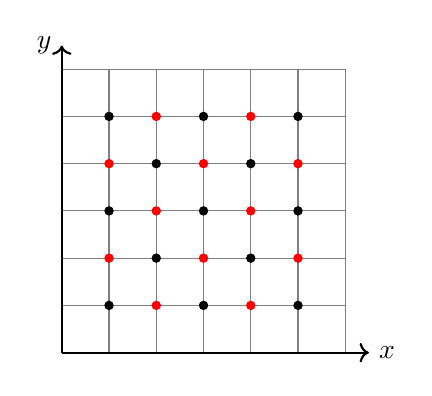
\begin{tikzpicture}[scale=0.6]
        % Draw horizontal lines
        \foreach \y in {0,1,...,6} {
            \draw[gray, thin] (0,\y) -- (6,\y);
        }
        % Draw vertical lines
        \foreach \x in {0,1,...,6} {
            \draw[gray, thin] (\x,0) -- (\x,6);
        }
        % Optionally, add axes
        \draw[thick,->] (0,0) -- (6.5,0) node[right] {$ x $};
        \draw[thick,->] (0,0) -- (0,6.5) node[left] {$ y $};
        
        % Draw filled circles at internal grid points with alternating colors
        \foreach \x in {1,2,...,5} {
            \foreach \y in {1,2,...,5} {
                \pgfmathparse{mod(\x+\y,2) ? "red" : "black"}
                \edef\circlecolor{\pgfmathresult}
                \fill[\circlecolor] (\x,\y) circle (0.1);
            }
        }
    \end{tikzpicture}
    \caption{红黑排序}
    \label{Red-Black}
\end{figure}

对于SOR迭代,迭代矩阵为$ G^{\omega} = (D-\omega L)^{-1}[(1-\omega) D + \omega U] $,于是$ G^\omega x = \lambda x $等价于
\[
    [(\lambda + \omega - 1)D - \lambda \omega L - \omega U]x = 0,
\]
对于模型问题,SOR迭代的特征值问题为
\[
    \begin{cases}
        (\lambda+\omega-1)u_{ij} - \frac{\omega}{4}(\lambda u_{i-1,j} + \lambda u_{i+1,j} + u_{i,j-1} + u_{i,j+1}) = 0, & 1\leqslant i,j\leqslant n-1,\\
        u_{i0} = u_{in} = u_{0j} = u_{nj} = 0,
    \end{cases}
\]
现在我们来讨论$ \lambda^{JA} $与$ \lambda^{\rm SOR} $之间的关系。令上式中的$ u_{ij} = (\pm \lambda^{\frac{1}{2}})^{i+j} V_{ij} $,于是$ \lambda\ne 0 $时有
\[
    \mu V_{ij} - \frac{1}{4}(V_{i-1,j}+V_{i,j-1}+V_{i+1,j}+V_{i,j+1})=0,\quad \mu = \pm \frac{\lambda + \omega - 1}{\omega \lambda^{\frac{1}{2}}},
\]
上式与Jacobi迭代的特征值问题形式相同,所以我们有
\[
    \lambda^{JA} = \pm \frac{\lambda^{\rm SOR} + \omega - 1}{\omega \sqrt{\lambda^{\rm SOR}} },
\]
从上式可以解出
\[
    \lambda^{\rm SOR}_{\pm} = \left( \frac{\lambda^{JA}\omega}{2} \pm \sqrt{(\frac{\lambda^{JA}\omega}{2})^2 - (\omega-1)}  \right)^2,
\]
因此$ \lambda^{\rm SOR} $可以视作$ \lambda^{JA} $和$ \omega $的函数,记为$ \lambda^{\rm SOR}(\lambda^{JA}, \omega) $,并令
\[
    \Lambda^{\rm SOR}(\lambda^{JA}, \omega) = \max\{\lambda_+^{\rm SOR}(\lambda^{JA}, \omega),\lambda_-^{\rm SOR}(\lambda^{JA}, \omega)\}.
\]
可以证明
\[
    \Lambda^{\rm SOR}(\lambda^{JA}, \omega) = 
    \begin{cases}
        \lambda_+^{\rm SOR}(\lambda^{JA}, \omega), & 0< \omega\leqslant \omega(\lambda^{JA}),\\
        \omega-1, & \omega(\lambda^{JA}) < \omega <2,
    \end{cases}
\]
其中
\[
    \omega(\lambda^{JA}) = \frac{2}{1 + \sqrt{1-(\lambda^{JA})^2} }
\]
是使之前$ \lambda^{JA} $和$ \lambda^{\rm SOR} $满足的二次方程的判别式$ (\lambda^{JA}\omega / 2)^2 - (\omega-1) = 0 $的在$ (0,2) $之间的根。分析可知如下事实:
\begin{itemize}
    \item 当固定$ \lambda^{JA} $,令$ \omega $变化时,$ \Lambda^{\rm SOR}(\lambda^{JA}, \omega) $在$ \omega $从$ 0 $变化到$ \omega(\lambda^{JA}) $时单调减少,在$ \omega = \omega(\lambda^{JA}) $时取到最小值,在$ \omega(\lambda^{JA}) $处的左侧导数为$ -\infty $,而在$ \omega(\lambda^{JA}) < \omega <2 $上等于$ \omega-1 $单调增加;
    \item 当固定$ \omega $,令$ \lambda^{JA} $变化时,$ \Lambda^{\rm SOR}(\lambda^{JA}, \omega) $是关于$ \lambda^{JA} $的增函数。
\end{itemize}
不同的$ \lambda^{JA} $下$ \Lambda^{\rm SOR}(\lambda^{JA}, \omega) $随$ \omega $的变化情况如图\ref{fig:SORfactor}所示,其中
\[
    \omega_{\rm opt} = \frac{2}{1+ \sqrt{1-\rho(G^{JA})^2} }
\]
称为最佳收敛因子,当$ \omega = \omega_{\rm opt} $时$ \rho(G^\omega) $取到最小值
\[
    \rho(G^{\omega_{\rm opt}}) = \frac{1-\sqrt{1-\rho(G^{JA})^2}}{1+\sqrt{1-\rho(G^{JA})^2} },
\]
于是SOR迭代的最佳渐进收敛速度为
\[
    R_\infty(G^{\omega_{\rm opt}}) = -\ln\rho(G^{\omega_{\rm opt}}) = -\ln \frac{1-\sqrt{1-\rho(G^{JA})^2}}{1+\sqrt{1-\rho(G^{JA})^2} },
\]
在模型问题中$ \rho(G^{JA}) = \cos(h \pi) $,所以SOR迭代的最佳渐进收敛速度在模型问题中为
\[
    R_\infty(G^{\omega_{\rm opt}}) = -\ln \frac{1-\sin(h \pi)}{1+\sin(h \pi)}\sim 2h \pi,\quad h\to 0,
\]
由此可见SOR的收敛速度往往比Jacobi迭代和G-E要快得多。
\begin{figure}[htpb]
    \centering
    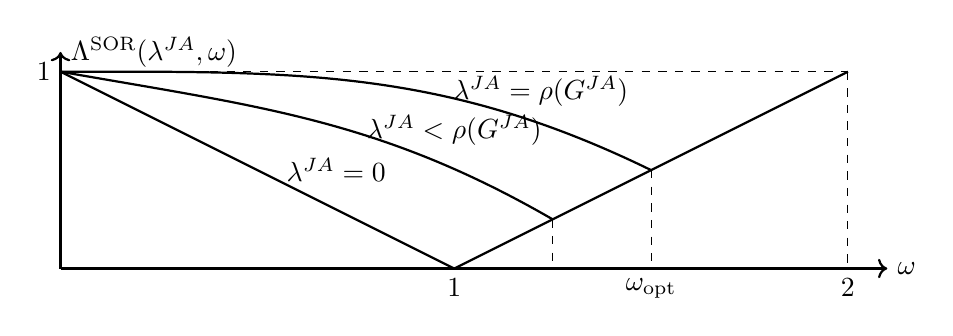
\begin{tikzpicture}[scale=0.5]
        % Draw axes
        \draw[thick,->] (0,0) -- (21,0) node[right] {$ \omega $};
        \draw[thick,->] (0,0) -- (0,5.5) node[right] {$ \Lambda^{\rm SOR}(\lambda^{JA}, \omega) $};
        \node[left] at (0,5) {1};
    
        % Draw main lines
        \draw[thick] (0,5) -- (10,0) node[below] {1};
        \draw[thick] (10,0) -- (20,5);
    
        % Draw curves
        \draw[thick] (0,5) to[out=0,in=154] (15,2.5);
        \node at (12.2,4.5) {$ \lambda^{JA} = \rho(G^{JA}) $};
        \draw[thick] (0,5) to[out=-10,in=150] (12.5,1.25);
        \node at (10,3.5) {$ \lambda^{JA} < \rho(G^{JA}) $};
        \node at (7,2.5) {$ \lambda^{JA} = 0 $};
    
        % Draw dashed lines
        \draw[dashed] (20,5) -- (20,0) node[below]{2};
        \draw[dashed] (15,2.5) -- (15,0) node[below]{$ \omega_{\rm opt} $};
        \draw[dashed] (12.5,1.25) -- (12.5,0);
        \draw[dashed] (0,5) -- (20,5);
    
    \end{tikzpicture}
    \caption{不同的$ \lambda^{JA} $下$ \Lambda^{\rm SOR}(\lambda^{JA}, \omega) $随$ \omega $的变化情况}
    \label{fig:SORfactor}
\end{figure}

\subsection{误差分析}
由于数值计算会引入舍入误差,所以在一些情况下,即使理论上迭代法是收敛的,但在实际计算中可能出现结果却是发散的现象,因此在对算法进行收敛性分析之外还必须进行误差分析。按照惯例,迭代法的误差分析分为前向误差分析和后向误差分析两部分。

\subsubsection{前向误差分析}

由于单步线性定常迭代法的迭代格式为
\[
    Mx^{(k+1)} = Nx^{(k)} + b,
\]
不难得到浮点计算下求解上述系统得到的数值解$ \hat{x}^{(k)} $满足如下后向误差关系
\begin{equation}
    (M+\Delta M^{(k+1)})\hat{x}^{(k+1)} = N\hat{x}^{(k)} + b + f_k,
\end{equation}
其中$ f_k $是在计算$ N\hat{x}^{(k)}+b $时引入的误差,而$ \Delta M^{(k+1)} $则来自于求解线性系统$ M x = N\hat{x}^{(k)} + b + f_k $。为了将这两部分后向误差分离出来,我们可以将上式重写为
\begin{equation}\label{eq:recurrence}
    M \hat{x}^{(k+1)} = N\hat{x}^{(k)} + b - \xi^{(k)},
\end{equation}
其中
\[
    \xi^{(k)} = -f_k + \Delta M^{(k+1)}\hat{x}^{(k+1)}.
\]
当使用Jacobi迭代、G-E迭代和SOR迭代时,$ M $是三角矩阵,因此$ |\Delta M^{(k+1)}|\leqslant c'_n u |M| $,于是我们有
\begin{equation}
    |\xi^{(k)}|\leqslant c_n u (|M| |\hat{x}^{(k+1)}| + |N| |\hat{x}^{(k)}| + |b|) :=\textcolor{blue}{\mu^{(k)}}.
\end{equation}
根据迭代关系式\eqref{eq:recurrence},我们有
\begin{equation}
    \hat{x}^{(m+1)} = G^{m+1}x_0 + \sum_{k=0}^m G^k M^{-1}(b - \xi^{(m-k)}),
\end{equation}
而准确解$ x^* $满足
\[
    x^* = G^{m+1}x^* + \sum_{k=0}^m G^k M^{-1}b,
\]
于是误差向量$ e^{(m+1)} = \hat{x}^{(m+1)} - x^* $满足
\begin{equation}
    e^{(m+1)} = G^{m+1}e^{(0)} - \sum_{k=0}^m G^k M^{-1}\xi^{(m-k)},
\end{equation}
进而数值上的前向误差满足
\begin{equation}
    |e^{(m+1)}|\leqslant |G^{m+1}e^{(0)}| + \sum_{k=0}^m |G^k M^{-1}||\xi^{(m-k)}| = \textcolor{red}{|G^{m+1}e^{(0)}|} + \textcolor{red}{\sum_{k=0}^m |G^k M^{-1}|\mu^{(m-k)}}.
\end{equation}
因此理论上的收敛性条件$ \rho(G)<1 $实际上只保证了上式中第一项$ |G^{m+1}e^{(0)} |$在$ m $足够大时趋于0,而数值上的稳定性还需要让第二项$ \sum_{k=0}^m |G^k M^{-1}|\mu^{(m-k)} $同时也足够小,下面的分析将围绕这一点展开。

首先我们来进行范数意义下的前向误差分析,令
\[
    \tau_{x^*} = \sup_k \frac{\| \hat{x}^{(k)} \|_\infty}{\| x^* \|_\infty},
\]
则
\[
    \begin{aligned}
        \| e^{(m+1)} \|_\infty \leqslant & \| G^{m+1} e^{(0)} \|_\infty + \sum_{k=0}^m \| G^k M^{-1} \|_\infty \| \mu^{(m-k)} \|_\infty\\
        \leqslant &\| G^{m+1} e^{(0)} \|_\infty + \max_{0\leqslant k\leqslant m} \| \mu^{(m-k)} \|_\infty\cdot\sum_{k=0}^m \| G^k M^{-1} \|_\infty \\
        \leqslant &\| G^{m+1} e^{(0)} \|_\infty + c_n u (1+\tau_{x^*})(\| M \|_\infty + \| N \|_\infty)\| x^* \|_\infty \cdot \sum_{k=0}^m \| G^kM^{-1} \|_\infty,
    \end{aligned}
\]
其中第三行的不等号来自于
\[
    \| \mu^{(k)} \|_\infty \leqslant c_n u(\| M \|_\infty \| \hat{x}^{(k+1)} \|_\infty + \| N \|_\infty \| \hat{x}^{(k)} \|_\infty + \| b \|_\infty),
\]
而$ \| \hat{x}^{(k)} \|_\infty \leqslant \tau_{x^*} $,$ \| b \|_\infty = \| (M-N)x^* \|_\infty \leqslant (\| M \|_\infty + \| N \|_\infty)\| x^* \|_\infty $。
如果$ \| G \|_\infty = q<1 $,则
\begin{equation}
    \textcolor{red}{\| e^{(m+1)} \|_\infty \leqslant \| G^{m+1} e^{(0)} \|_\infty + c_n u (1+\tau_{x^*})(\| M \|_\infty + \| N \|_\infty)\| x^* \|_\infty \cdot \frac{\| M^{-1} \|_\infty}{1-q}}.
\end{equation}
这一结果对应于定理\ref{th:theoryerror}中的理论误差估计。从上式中可以看出,当$ q $足够远离$ 1 $,并且$ \tau_{x^*} $和$ \| M^{-1} \|_\infty $不是太大时,前向误差对于足够大的$ m $来说是一个较小的量。

为了进行分量意义下的误差估计,令
\[
    \theta_{x^*} = \sup_k \max_{1\leqslant i\leqslant n}\left( \frac{|\hat{x}^{(k)}_i|}{|x^*_i|} \right),
\]
为了避免$ 0 $做分母,上面的定义可以修改为
\[
    \theta_{x^*} = \sup_k \max_{1\leqslant i\leqslant n}\left( \frac{ [(|M|+|N|)|\hat{x}^{(k)}|]_i}{[(|M|+|N|)|x^*|]_i} \right),
\]
于是与之前类似地有
\[
    |\mu^{(k)}| \leqslant c_n u(1+\theta_{x^*})(|M|+|N|)|x^*|,
\]
进而
\[
    |e^{(m+1)}|\leqslant |G^{m+1} e^{(0)}| + c_n u(1+\theta_{x^*}) \left( \sum_{k=0}^\infty |G^kM^{-1}| \right)  (|M|+|N|)|x^*|.
\]
注意到$ A = M-N = M(I-M^{-1}N) $,因此当$ \| G=M^{-1}N \|_\infty = q<1 $时
\[
    A^{-1} = (I-G)^{-1}M^{-1} = \sum_{k=0}^\infty G^k M^{-1}.
\]
因此$ \sum_{k=0}^\infty |G^kM^{-1}| \geqslant |A^{-1}| $,于是我们定义两者的比值为
\[
    c(A) = \min\left\{ \epsilon:\sum_{k=0}^\infty |G^kM^{-1}| \leqslant \epsilon \left\vert \sum_{k=0}^\infty G^kM^{-1} \right\vert = \epsilon|A^{-1}| \right\} ,
\]
所以最终分量意义下的前向误差估计为
\begin{equation}\label{eq:componenterror}
    \textcolor{red}{|e^{(m+1)}|\leqslant |G^{m+1} e^{(0)}| + c_n u(1+\theta_{x^*}) c(A)|A^{-1}|  (|M|+|N|)|x^*|}.
\end{equation}
上式中的$ c(A) $只有在$ \rho(G) $非常接近$ 1 $时会变得很大,实际上我们有如下估计
\[
    c(A) \geqslant \max_i \frac{|1-\lambda_i|}{1-|\lambda_i|},\quad \lambda_i\in \Lambda(G),
\]
只有当$ c(A) $不太大时(通常$ O(n) $),此时$ \rho(G) $才能足够地远离1,本节的古典迭代法才能在理论收敛的情况下具有数值稳定性,为此我们将\eqref{eq:componenterror}改写成
\begin{equation}
    \|e^{(m+1)}\|_\infty \leqslant \|G^{m+1} e^{(0)}\|_\infty + c_n u(1+\theta_{x^*}) c(A)\| |A^{-1}|  (|M|+|N|)|x^*| \|_\infty,
\end{equation}
注意到对于Jacobi迭代或者G-E迭代的方法而言$ |M|+|N| = |M-N| = |A| $,因此上式变为
\[
    \textcolor{red}{\|e^{(m+1)}\|_\infty \leqslant \|G^{m+1} e^{(0)}\|_\infty + c_n u(1+\theta_{x^*}) c(A) {\rm cond}(A,x)},
\]
所以当$ \theta_{x^*}c(A) = O(1) $时,Jacobi迭代或者G-E迭代在分量意义下是前向稳定的。对于其他的算法,如果$ |M|+|N|\leqslant \alpha |A| $,其中$ \alpha=O(1) $,则有类似的结论。例如考虑SOR,有
\[
    M = \frac{1}{\omega}(D+\omega L), \quad N = \frac{1}{\omega}[(1-\omega)D - \omega U],
\]
于是
\[
    |M|+|N|\leqslant \frac{1+|1-\omega|}{\omega}|A| = f(\omega)|A|,
\]
其中$ f(\omega) $在$ \omega\in(0,1) $上从$ \infty $单调下降到$ 1 $,在$ (1,2) $上恒为$ 1 $,因此SOR的前向误差估计为
\[
    \textcolor{red}{\|e^{(m+1)}\|_\infty \leqslant \|G^{m+1} e^{(0)}\|_\infty + c_n u(1+\theta_{x^*}) c^{\rm SOR}(A)f(\omega) {\rm cond}(A,x)}.
\]

\subsubsection{后向误差分析}
现在考虑残差向量$ r^{(k)} = b - A \hat{x}^{(k)} $,希望找到它的一个上界。首先因为$ r^{m+1}= A(x^* - x^{(m+1)}) = -A e^{(m+1)} $有
\[
    r^{(m+1)}  = AG^{m+1}(x^* - x^{(0)})+\sum_{k=0}^m AG^k M^{-1}\xi^{(m-k)},
\]
注意到
\[
    AG = (M-N)M^{-1}N = N-NM^{-1}N = NM^{-1}(M-N) = NM^{-1}A,
\]
若记$ H = NM^{-1} $,则$ AG = HA $,进而$ AG^k = H^kA $,于是
\[
    \begin{aligned}
        r^{(m+1)} &= H^{m+1}A(x^* - x^{(0)})+\sum_{k=0}^m H^k AM^{-1}\xi^{(m-k)}\\
        &=H^{m+1}r^{(0)} + \sum_{k=0}^m H^k (I - H)\xi^{(m-k)},
    \end{aligned}
\]
与上一小节类似地可得
\begin{equation}\label{eq:backerror}
    \| r^{(m+1)} \|_\infty \leqslant \| H^{m+1} r^{(0)} \|_\infty + c_n u \sigma(1+\tau_{x^*})(\| M \|_\infty + \| N \|_\infty)\| x \|_\infty,
\end{equation}
其中
\[
    \sigma = \| \sum_{k=0}^\infty |H^k (I-H) \| .
\]
注意到如果$ \| H \|_\infty<1 $则
\[
    \sigma\leqslant \| I-H \|_\infty \sum_{k=0}^\infty \| H \|_\infty^k = \frac{\| I-H \|_\infty}{1-\| H \|_\infty},
\]
因此$ \| H \|_\infty = q<1 $时因子$ \sigma $具有一个较好的上界。进一步地,如果$ H $可以对角化,即$ P^{-1}HP = \Lambda $,则$ \sigma $有更小的界
\[
    \begin{aligned}
        \sigma &= \| \sum_{k=0}^\infty |P(\Lambda^k - \Lambda^{k+1})P^{-1}| \|_\infty\\
        &\leqslant \| |P| \sum_{k=0}^\infty \operatorname{diag}(|1-\lambda_i||\lambda_i^k|)| |P^{-1}| \|_\infty\\
        &= \| |P| \operatorname{diag}(\frac{|1-\lambda_i|}{1-|\lambda_i|}) |P^{-1}| \|_\infty\\
        &\leqslant \kappa_\infty(P) \max_i \frac{|1-\lambda_i|}{1-|\lambda_i|}.
    \end{aligned}
\]
其中的$ \lambda_i $是$ H $的特征值,注意到$ \lambda_i(H) = \lambda_i(NM^{-1}) = \lambda_i(M^{-1}N) = \lambda_i(G) $,因此上述误差界中的$ \max_i |1-\lambda_i| /(1-|\lambda_i|) $与$ c(A) $的上界一致。

之前已经证明对于系统$ Ax=b $的求解而言,后向误差满足
\begin{equation}
    \eta_{E,f}(y) = \frac{\| b - Ay \|}{\| E \| \| y \| + \| f \|},
\end{equation}
而
\[
    \frac{(\| M \|_\infty + \| N \|_\infty) \| x \|_\infty}{\| A \|_\infty \| \hat{x}^{(m)} \|_\infty + \| b \|_\infty} =  \frac{\| M \|_\infty + \| N \|_\infty}{\| A \|_\infty} \cdot \frac{\| A \|_\infty \| x \|_\infty}{\| A \|_\infty \| \hat{x}^{(m)} \|_\infty + \| b \|_\infty},
\]
所以根据\eqref{eq:backerror}可知,对于足够大的$ m $,无穷范数下的后向误差满足如下关系
\begin{equation}
    \eta_{A,b}(\hat{x}^{(m)}) \leqslant c_n u(1+\tau_{x^*})\sigma\left( \frac{\| M \|_\infty + \| N \|_\infty}{\| A \|_\infty} \right) ,
\end{equation}
对于Jacobi迭代、G-E迭代以及$ \omega\in(1,2) $的SOR,$ \| M \|_\infty + \| N \|_\infty \leqslant 2\| A \|_\infty $,因此这三种方法在$ \sigma $比较小时在范数意义下是后向稳定的。

\section{现代迭代法——空间投影}
区别于上一节的古典迭代法使用的矩阵分割,多数现代的迭代法是基于子空间投影的,这些方法在某些子空间中搜索修正项,随着子空间的维数增加越来越接近整个空间,得到的近似解也就越来越接近真实解。

\subsection{投影方法}
给定某一线性系统$ Ax=b $,其中$ A $是$ n $阶方阵。投影方法的基本想法是:选定原本解空间$ \mathbb{R}^n $的一个$ m $维的子空间$ \mathcal{K} $,在该空间内寻找问题的近似解$ \tilde{x} $。为了确定该近似解,我们需要$ m $个线性无关的约束条件以在$ m $维的空间$ \mathcal{K} $中找到它,通常的做法是要求满足\emph{Petrov-Galerkin条件(P-G)},即残差向量$ b-A \tilde{x} $与$ m $个线性无关的向量都正交,这$ m $个向量张成的空间记作$ \mathcal{L} $,即
\[
    \text{Find } \tilde{x}\in \mathcal{K},\quad s.t.\quad b - A\tilde{x}\perp \mathcal{L}.
\]
为了利用已有的初始向量$ x^{(0)} $的先验信息,通常我们不直接在$ \mathcal{K} $中寻找$ \tilde{x} = x^{(1)} $,而是在$ x^{(0)} + \mathcal{K} $中寻找$ \tilde{x} $,即
\begin{equation}
    \text{Find } x^{(1)}\in x^{(0)} + \mathcal{K},\quad s.t.\quad b - Ax^{(1)}\perp \mathcal{L}.
\end{equation}
我们称$ \mathcal{K} $是这一方法的搜索空间,而$ \mathcal{L} $是该方法的约束空间。如果记从$ x^{(0)} $到$ x^{(1)} $的修正项为$ \delta $,即$ x^{(1)} = x^{(0)} + \delta $,则残差$ r^{(1)} = r^{(0)} - A\delta $,上面的问题等价于
\[
    \text{Find } \delta\in \mathcal{K},\quad s.t.\quad r_0 - A \delta\perp \mathcal{L},
\]

现在我们将上述要求写成矩阵形式。令$ V = (v_1, v_2,\cdots ,v_m) $和$ W = (w_1,w_2,\cdots ,w_m) $分别是以$ \mathcal{K} $和$ \mathcal{L} $的一组基组成的$ n\times m $阶矩阵,于是有$ \delta = Vy\in \mathcal{K} $,其中$ y\in \mathbb{R}^m $。由于$ r^{(0)} - A\delta\perp \mathcal{L} $等价于$ r^{(1)} $正交于$ \mathcal{L} $的每一个基向量,即$ W^Tr^{(1)} = 0 $,而
\[
    W^T (r^{(0)} - A\delta) = 0 \iff W^T r^{(0)} = W^T A V y,
\]
由于$ W^T A V $是$ m $阶方阵,所以上式右端是一个$ m $维的线性方程组,解得$ y $即可得到$ \delta $,进而得到下一个近似解
\begin{equation}\label{eq:generalprojection}
    x^{(1)} = x^{(0)} + \delta = x^{(0)} + V(W^TAV)^{-1}W^T r^{(0)}.
\end{equation}
为了保证$ W^T A V $的可逆性,有两种特殊的情况特别重要:
\begin{enumerate}
    \item $ A\in \mathcal{S}_{++} $并且$ \mathcal{L} = \mathcal{K} $;
    \item $ A $非奇异并且$ \mathcal{L} = A\mathcal{K} $。
\end{enumerate}
在这两种情况下,无论$ V $和$ W $如何选取,$ W^T A V $都是可逆的。

根据约束空间与搜索空间之间的关系,投影方法可以分为两类:$ \mathcal{K} = \mathcal{L} $时称为\emph{正交(orthogonal)投影方法},此时P-G条件也被直接称作Galerkin条件,并且可以选取同一组向量充当$ \mathcal{K} $和$ \mathcal{L} $的基,于是$ V=W $;当$ \mathcal{K} \ne \mathcal{L} $时称为\emph{倾斜(oblique)投影方法}。

\subsubsection{投影矩阵}
如果方阵$ P $满足$ P^2 = P $,则称$ P $是一个投影矩阵。由$ \lambda x =Px = P^2 x=\lambda Px = \lambda^2 x $可知$ P $的特征值为$ 0 $或$ 1 $,于是$ {\rm Rank}(P) = {\rm Tr}(P) $,并且算子范数$ \| P \|_2 = 1 $(当$ P $不是零矩阵),一般地对于相容的矩阵范数有$ \| P \| =\| P^2 \| \leqslant \| P \|^2 $,于是$ \| P \|\geqslant 1 $。投影矩阵分为正交投影矩阵和斜投影矩阵,如果$ P^2=P $满足
\[
    (Px,(I-P)x) = 0, \quad \forall x,
\]
则称$ P $是正交投影矩阵,否则称为斜投影矩阵。

如果某一子空间$ M $有一组单位正交基$ \{u_1,u_2,\cdots ,u_m\} $,记$ U = (u_1,u_2,\cdots ,u_m) $,则从$ \mathbb{C}^n $到$ M $的正交投影算子$ P $可以表示为
\begin{equation}
    P = UU^* = \sum_{i=1}^m (u_i, \cdot) u^i.
\end{equation}
而如果$ \{v_1, v_2,\cdots ,v_m\} $只是$ M $的一组不一定正交的基,则$ P $可以表示为
\begin{equation}
    P = V(V^*V)^{-1}V^*,
\end{equation}
其中$ V = (v_1,v_2,\cdots ,v_m) $,$ (V^*V)^{-1} $起到正则化的作用。由此可见正交投影矩阵$ P $和$ I-P $都是对称的。

一般地,如果$ D\in \mathcal{S}_{++} $,则它可以诱导出一个内积$ (x,y)_D = (Dx,y) $,并导出一个范数$ \| x \|_D = (x,x)_D^{1 / 2} $,则子空间$ M $上的投影算子$ P_D $满足
\begin{equation}
    x = P_D x^* \iff \min_{x\in M} \| x^* - x \|_D,
\end{equation}
记$ M $的一组基组成的矩阵为$ V $,于是$ x=Vy\in M $,令$ D_y\| x^* - x \|_D^2=0 $可得$ P_D $的矩阵表示为
\begin{equation}
    P_D = V(V^TDV)^{-1}V^TD,
\end{equation}
它满足
\begin{equation}
    (P_Dx, (I-P_D)x)_D = 0,\quad \forall x.
\end{equation}
当$ D = I $时,$ P_D $是正交投影算子,否则是斜投影算子,称为$ D $-投影算子。

如果给定矩阵$ V $和$ U $,它们的列向量分别张成了投影的目标子空间$ \mathcal{K} $和方向子空间$ \mathcal{L} $(即投影方向,$ I-P $与$ \mathcal{L} $正交),则相应的斜投影矩阵为:
\begin{equation}
    P = V(U^TV)^{-1}U^T,
\end{equation}
满足
\[
    R(P)\subseteq \mathcal{K},\quad R(I-P)\perp \mathcal{L},
\]
因此要寻找$ x^{(1)} = x^{(0)} + \delta $,其中$ \delta\in \mathcal{K} $,满足$ b-Ax^{(1)}\perp \mathcal{L} $,只需要找到某个如上形式的斜投影矩阵$ P $,要求存在$ y $使得
\[
    r^{(1)} = r^{(0)} -A \delta = A(e^{(0)}-\delta) = (I-P)y.
\]

\subsubsection{最优化形式}
本小节需要使用到如下引理。
\begin{lemma}
    给定$ A\in \mathcal{S}_{++} $,令$ P_{M,A}: \mathbb{C}^n\to M $是由$ A $-内积诱导的到子空间$ M $上的投影算子(正交投影$ P_{M,I} $简记为$ P_M $),则任意$ x\in \mathbb{C}^n $都有
    \begin{equation}
        \min_{y\in M} \| x-y \|_A = \| x-y^* \|_A \iff y^* = P_{M,A}x,\text{ that is }
        \begin{cases}
            y^*\in M,\\
            x-y^*\perp_A M.
        \end{cases}
    \end{equation}
\end{lemma}
使用上面的引理,可以将$ b-Ax^{(1)}\perp \mathcal{L} $的条件在之前提到的两种特殊情况下写成最优化形式:
\begin{theorem}
    要求$ x^{(1)} = x^{(0)}+\delta $,其中$ \delta\in \mathcal{K} $,则如下结论成立:
    \begin{enumerate}
        \item 当$ A\in \mathcal{S}_{++} $并且$ \mathcal{L} = \mathcal{K} $时
        \begin{equation}
            b-Ax^{(1)}\perp \mathcal{L} = \mathcal{K} \iff E(x^{(1)}) = \min_{x\in x^{(0)}+\mathcal{K}} E(x) \iff \delta = P_{\mathcal{K},A} e^{(0)},
        \end{equation}
        其中
        \[
            E(x) = \| x^* - x \|_A = (A(x^* - x), x^* - x)^{\frac{1}{2}},\quad e^{(i)} = x^* - x^{(i)}.
        \]
        \item 当$ A $是任意方阵并且$ \mathcal{L} = A\mathcal{K} $时
        \begin{equation}
            b-Ax^{(1)}\perp \mathcal{L} = A \mathcal{K} \iff R(x^{(1)}) = \min_{x\in x^{(0)}+\mathcal{K}} R(x)\iff A \delta = P_{A\mathcal{K}} r^{(0)},
        \end{equation}
        其中
        \[
            R(x) = \| b - Ax \|_2 = (A(x^*-x), A(x^*-x))^{\frac{1}{2}}.
        \]
    \end{enumerate}
\end{theorem}
在第二种情况下,即$ \mathcal{L} = A \mathcal{K} $时,$ r^{(1)} = b-Ax^{(1)} = r^{(0)} - A \delta $,定理的结论表明$ A \delta $是$ r^{(0)} $在$ A\mathcal{K} = \mathcal{L} $上的正交投影,即
\[
    A \delta = P_{A\mathcal{K}} r^{(0)}, \quad r^{(1)} = r^{(0)} -  A \delta = (I-P_{A\mathcal{K}}) r^{(0)}.
\]
其中$ P_{A\mathcal{K}} $是$ A\mathcal{K} $上的正交投影算子,满足
\[
    (P_{A\mathcal{K}}x, (I-P_{\mathcal{K}})x) = 0,\quad \forall x.
\]
另外,在定理的第二种情况下没有要求$ A $是非奇异的,当$ A $是奇异的时候,定理的结论仍然成立,但是最优的$ \delta $不唯一。

在第一种情况下,即$ \mathcal{L} = \mathcal{K} $时,$ e^{(1)} = x^* - x^{(1)} = e^{(0)} - \delta $,定理的结论表明$ \delta $是$ e^{(0)} $在$ \mathcal{K} = \mathcal{L} $上的$ A $-投影,$ \delta = P_{\mathcal{K},A} d^{(0)} $,其中$ P_{\mathcal{K},A} $是$ \mathcal{K} $上的$ A $-投影算子,满足
\[
    (P_{\mathcal{K}, A}x, (I-P_{\mathcal{K}, A})x)_A := (AP_{\mathcal{K}, A}x, (I-P_{\mathcal{K}, A})x) = 0,\quad \forall x.
\]

这两种情况分别对应两类重要的迭代方法:
\begin{enumerate}
    \item $ A\in \mathcal{S}_{++} $并且$ \mathcal{L} = \mathcal{K} $:
    \begin{equation}
        e^{(1)} = (I - P_{\mathcal{K}, A})e^{(0)},
    \end{equation}
    并且$ \| e^{(1)} \|_A \leqslant \| e^{(0)} \|_A $,其中$ P_{\mathcal{K}, A} $是$ \mathcal{K} $上的$ A $-投影算子。这种情况对应\emph{误差投影方法};
    \item $ A $是任意方阵并且$ \mathcal{L} = A\mathcal{K} $:
    \begin{equation}
        r^{(1)} = (I - P_{A\mathcal{K}})r^{(0)},
    \end{equation}
    并且$ \| r^{(1)} \|_2 \leqslant \| r^{(0)} \|_2 $,其中$ P_{A\mathcal{K}} $是$ A\mathcal{K} $上的正交投影算子。这种情况对应\emph{残差投影方法}。
\end{enumerate}
\subsubsection{投影法的矩阵表示和误差界}
\eqref{eq:generalprojection}已经给出了投影法更新格式的一种矩阵表示,本节我们使用投影算子给出更一般的格式。构造一种投影法,等价于给定$ \mathcal{K},\mathcal{L} $,令$ P_{\mathcal{K}} $为到$ \mathcal{K} $上的正交投影算子,以及$ Q_{\mathcal{K}}^{\mathcal{L}} $为某个到$ \mathcal{K} $上的斜投影算子,满足
\[
    (I - Q_{\mathcal{K}}^{\mathcal{L}})x \perp \mathcal{L},\quad \forall x\in \mathbb{C}^n.
\]
于是要让$ b - A x^{(1)}\perp \mathcal{L} $只需
\[
    \exists y\in \mathbb{C}^n \text{ s.t. } (I-Q_{\mathcal{K}}^{\mathcal{L}})y = r^{(1)} = b-Ax^{(1)},
\]
在上式左端两侧同时左乘$ Q_{\mathcal{K}}^{\mathcal{L}} $,有
\[
    Q_{\mathcal{K}}^{\mathcal{L}}(I - Q_{\mathcal{K}}^{\mathcal{L}})y = Q_{\mathcal{K}}^{\mathcal{L}} (b-Ax^{(1)}),
\]
由于$ Q_{\mathcal{K}}^{\mathcal{L}} $是投影矩阵,所以上式左端为$ 0 $,进而约束条件就变为了
\begin{equation}
    Q_{\mathcal{K}}^{\mathcal{L}} (b-Ax^{(1)}) = 0.
\end{equation}
当$ x^{(0)} = 0 $时,为了保证$ \delta = x^{(1)}\in \mathcal{K} $,实际上需要求解的是如下系统
\begin{equation}
    Q_{\mathcal{K}}^{\mathcal{L}} (b-AP_{\mathcal{K}}x) = 0,
\end{equation}
其中$ P_{\mathcal{K}}x = \delta $,上式等价于如下$ m $阶线性方程组
\begin{equation}
    Q_{\mathcal{K}}^{\mathcal{L}}AP_{\mathcal{K}}x =  Q_{\mathcal{K}}^{\mathcal{L}}b.
\end{equation}
至此原本的$ n $阶问题被转化为了$ m $阶问题,这正是投影法的目标。一般地,当$ x^{(0)}\ne 0 $时,要求解的方程组变为
\begin{equation}
    Q_{\mathcal{K}}^{\mathcal{L}}(r^{(0)} - A \delta) = 0,\quad \delta\in \mathcal{K},
\end{equation}
等价于令$ P_{\mathcal{K}}z = \delta $,考虑
\begin{equation}
    \textcolor{red}{Q_{\mathcal{K}}^{\mathcal{L}}AP_{\mathcal{K}} z = Q_{\mathcal{K}}^{\mathcal{L}}r^{(0)},\quad z\in \mathbb{C}^n}.
\end{equation}

特别地,如果$ \mathcal{K} $在$ A $下保持不变,即$ A \mathcal{K} = \mathcal{K} $,并且$ b \in \mathcal{K} $,则在起始向量$ x^{(0)} = 0 $时,注意到$ Q_{\mathcal{K}}^{\mathcal{L}}|_{\mathcal{L}} = I_{\mathcal{L}} $,我们有$ Q_{\mathcal{K}}^{\mathcal{L}} (b-Ax^{(1)}) = b-Ax^{(1)} $,所以使用任意投影法都可以得到精确解$ x^{(1)} = x^* $满足$ A x^{(1)} = b $。当$ x^{(0)}\ne 0 $时,如果$ r^{(0)} = b - Ax^{(0)}\in \mathcal{K} $,则结论仍然成立。

注意到$ b\in \mathcal{K} $时
\[
    \begin{aligned}
        b - Q_{\mathcal{K}}^{\mathcal{L}}AP_{\mathcal{K}}x^*
        &= Q_{\mathcal{K}}^{\mathcal{L}}A (I - P_{\mathcal{K}})x^*\\
        &= Q_{\mathcal{K}}^{\mathcal{L}}A (I - P_{\mathcal{K}})\cdot [(I - P_{\mathcal{K}})x^*],
    \end{aligned}
\]
我们有如下结论:
\begin{theorem}
    令$ \gamma = \| Q_{\mathcal{K}}^{\mathcal{L}}A(I-P_{\mathcal{K}}) \|_2 $,如果$ b\in \mathcal{K} $,则当$ x^{(0)} = 0 $时,原方程的准确解$ x^* $在$ m $阶方程组
    \[
        Q_{\mathcal{K}}^{\mathcal{L}}AP_{\mathcal{K}}x =  Q_{\mathcal{K}}^{\mathcal{L}}b = b
    \]
    中的误差满足
    \begin{equation}
        \|  b - Q_{\mathcal{K}}^{\mathcal{L}}AP_{\mathcal{K}}x^* \|_2\leqslant \gamma \| (I-P_{\mathcal{K}})x^* \|_2.
    \end{equation}
\end{theorem}
\noindent 定理中$ \| (I-P_{\mathcal{K}})x^* \|_2 $是准确解$ x^* $距离$ \mathcal{K} $的距离。由于当$ x^{(0)} = 0 $时$ x^{(1)} \in P_{\mathcal{K}} $,所以
\[
    \| x^* - x^{(1)} \|_2 \geqslant \| (I-P_{\mathcal{K}})x^* \|_2 = \inf_{x\in \mathcal{K}} \| x^* - x \|_2.
\]
因此只有当选取的$ \mathcal{K} $足够接近$ x^* $时,投影法才能得到较好的近似解。
特别地,根据之前的回顾,当使用正交投影方法时,要求$ \mathcal{K} = \mathcal{L} $,如果$ \mathcal{K} $有一组单位正交基$ \{v_{1}, \cdots , v_{m}\} $,则$ P_{\mathcal{K}} = VV^* $,令$ W = V $,则$ Q_{\mathcal{K}}^{\mathcal{L}} = VV^* $,于是$ Q_{\mathcal{K}}^{\mathcal{L}}A P_{\mathcal{K}} = V(V^*AV)V^* $,上述定理的结论的矩阵形式为
\begin{equation}
    \| b - V(V^*AV)V^* x^* \|_2 \leqslant \gamma \| (I-P_{\mathcal{K}})x^* \|_2,
\end{equation}
因为$ b \in \mathcal{K} = A \mathcal{K} $有$ b = VV^* b $,所以
\[
    \| b - V(V^*AV)V^* x^* \|_2 = \| V^*b - (V^*AV)V^* x^* \|_2,
\]
进而有
\begin{equation}
    \| V^*b - (V^*AV)V^* x^* \|_2 \leqslant \gamma \| (I-P_{\mathcal{K}})x^* \|_2.
\end{equation}

\subsection{一维投影方法}
如果某种投影迭代法在每一次迭代时使用的搜索空间和约束空间都是一维的,即
\[
    \mathcal{K}_i = {\rm span}\{v\},\quad \mathcal{L}_i = {\rm span}\{w\},
\]
则称该迭代法是一种一维投影方法,这种方法每次的更新格式为
\begin{equation}
    x^{(i+1)} = x^{(i)} + \alpha_i v,
\end{equation}
其中$ \alpha $是某一待确定的常数,注意到P-G条件要求$ r^{(i)} - A \delta\perp w $可得
\[
    \alpha_i = \frac{(r^{(i)}, w)}{(Av, w)}.
\]

不难看出,由于Jacobi迭代中的每一次更新都要求
\[
    (b - Ax^{(k+i / n)})_i = 0 \iff b - Ax^{(k+i / n)} \perp e_i
\]
因此它的每次迭代都相当于在使用一维投影方法,其中$ \mathcal{K}_i = \mathcal{L}_i = \{e_i\} $,其中$ e_i $在$ i $到达$ n $之后重新回到$ 1 $进行循环,把第$ k+1 $次从$ 1 $到$ n $的循环中的更新量相加起来就得到了$ x^{(k+1)}-x^{(k)} $所需的更新量。G-E迭代和SOR迭代同样类似。

本小节我们给出三种经典常见的一维投影方法。
\subsubsection{最速下降法}
当$ A\in \mathcal{S}_{++} $时,在第$ i+1 $次迭代时,最速下降法选择$ v = w = r^{(i)} $,更新格式为
\begin{equation}
    x^{(i+1)} = x^{(i)} + \alpha_i r^{(i)},\quad \alpha_i = \frac{(r^{(i)}, r^{(i)})}{(Ar^{(i)}, r^{(i)})},
\end{equation}
因此这种方法是一种误差投影方法,在每一次迭代时都要求
\[
    \min_{x\in x^{(i)} + \mathcal{K}_i} \| x^* - x \|_A,
\]
等价于在寻找函数$ f(x) = \| x-x^* \|_A^2 $的极小值点时,在每一步更新时都沿着负梯度方向$ -\nabla f $下降,下降的长度$ \alpha $由一次线搜索找到当前方向上的极小值点来确定。
具体算法如\ref{alg:SDA}所示。
\begin{algorithm}[htbp]
    \caption{Steepest Descent Algorithm}\label{alg:SDA}
    \KwData{$ A\in \mathcal{S}_{++},b $ and initial guess $ x_0 $}
    \KwResult{An approximant solution $ x $.}
    $ x = x_0 $\;
    \While{Stop criterion is not satisfied}{
        $ r = b - Ax $\;
        $ \alpha = (r, r) / (Ar, r) $\;
        $ x = x + \alpha r $\;
    }
    \Return $ x $\;
\end{algorithm}

如下引理是经典的Kantorovich不等式。
\begin{lemma}
    给定任意$ A\in \mathcal{S}_{++} $,记$ \lambda_{\max} $和$ \lambda_{\min} $为$ A $的最大和最小特征值,则
    \begin{equation}
        \frac{\| x \|_A\cdot \| x \|_{A^{-1}}}{\| x \|_2^2}\leqslant \frac{\lambda_{\max}+\lambda_{\min}}{2\sqrt{\lambda_{\max}\lambda_{\min}} },\quad \forall x\ne 0.
    \end{equation}
\end{lemma}
\noindent 使用上述引理,我们可以得到最速下降法的收敛性定理,其中$ A $的正定性对于收敛而言是必要的。
\begin{theorem}
    对于任意$ A\in \mathcal{S}_{++} $,最速下降法的得到的近似解$ x^{(i)} $满足
    \begin{equation}
        \| x^{(i+1)} - x^* \|_A \leqslant \frac{\lambda_{\max} - \lambda_{\min}}{\lambda_{\max} - \lambda_{\min}} \| x^{(i)} - x^* \|_A,
    \end{equation}
    因此最速下降法是一种线性收敛的迭代方法。
\end{theorem}

\subsubsection{最小残差法}
如果$ A $不是正定的,但是$ A $的对称部分$ A^T+A $是正定的,则可以使用最小残差法。在第$ i+1 $次迭代时,最小残差法选择$ v = r^{(i)} $,$ w = A r^{(i)} $,更新格式为
\begin{equation}
    x^{(i+1)} = x^{(i)} + \alpha_i r^{(i)},\quad \alpha_i = \frac{(Ar^{(i)}, r^{(i)})}{(Ar^{(i)}, Ar^{(i)})},
\end{equation}
这种方法是一种残差投影方法,每一次迭代都要求
\[
    \min_{x\in x^{(i)} + \mathcal{K}_i} \| b - Ax \|_2,
\]
等价于在寻找函数$ f(x) = \| b - Ax \|_2^2 $的极小值点时,在每一步更新时都沿着残差方向$ r^{(i)} $下降,下降的长度$ \alpha $由一次线搜索找到当前方向上的极小值点来确定。具体算法如\ref{alg:MRA}所示。

\begin{algorithm}[htbp]
    \caption{Minimal Residual Algorithm}\label{alg:MRA}
    \KwData{$ A \text{ s.t. }A^T+A\in \mathcal{S}_{++},b $ and initial guess $ x_0 $}
    \KwResult{An approximant solution $ x $.}
    $ x = x_0 $\;
    \While{Stop criterion is not satisfied}{
        $ r = b - Ax $\;
        $ \alpha = (Ar, r) / (Ar, Ar) $\;
        $ x = x + \alpha r $\;
    }
    \Return $ x $\;
\end{algorithm}
\begin{theorem}
    如果$ A^T+A\in \mathcal{S}_{++} $,令
    \[
        \mu = \lambda_{\min}(\frac{A^T+A}{2}),\quad \sigma = \| A \|_2,
    \]
    则最小残差法的得到的近似解$ x^{(i)} $满足
    \begin{equation}
        \| b - Ax^{(i+1)} \|_2 \leqslant  (1-\frac{\mu^2}{\sigma^2})^{1 / 2} \| b - Ax^{(i)} \|_2,
    \end{equation}
    因此这种情况下最小残差法在使用任意初始向量$ x^{(0)} $时都是线性收敛的。
\end{theorem}

\subsubsection{残差下降法}
如果$ A $的对称部分不正定,但是$ A $是非奇异矩阵,则可以使用残差下降法。在第$ i+1 $次迭代时,残差下降法选择$ v = A^T r^{(i)} $,$ w = A r^{(i)} $,更新格式为
\begin{equation}
    x^{(i+1)} = x^{(i)} + \alpha_i A^T r^{(i)},\quad \alpha_i = \frac{(A^Tr^{(i)}, A^Tr^{(i)})}{(AA^Tr^{(i)}, A A^Tr^{(i)})},
\end{equation}
每一次迭代都要求
\[
    \min_{x\in x^{(i)} + \mathcal{K}_i} \| b - Ax \|_2,
\]
等价于在寻找函数$ f(x) = \| b - Ax \|_2^2 $的极小值点时,在每一步更新时都沿着负梯度方向$ -\nabla f $下降,下降的长度$ \alpha $由一次线搜索找到当前方向上的极小值点来确定。这种方法等价于对正规方程$ A^TAx=A^Tb $使用之前的最速下降法。
具体算法如\ref{alg:RSD}所示。

\begin{algorithm}[htbp]
    \caption{Residual Norm Steepest Descent Algorithm}\label{alg:RSD}
    \KwData{nonsingular $ A $, $ b $ and initial guess $ x_0 $}
    \KwResult{An approximant solution $ x $.}
    $ x = x_0 $\;
    $ r = b - Ax $\;
    \While{Stop criterion is not satisfied}{
        $ v = A^T r $\;
        $ \alpha = (v, v) / (Av, Av) $\;
        $ x = x + \alpha r $\;
        $ r = b - \alpha Av $\;
    }
    \Return $ x $\;
\end{algorithm}

\subsection{Krylov方法}

\subsubsection{Arnoldi算法}
\begin{algorithm}[htbp]
    \caption{Arnoldi's Procedure}\label{alg:Arnoldi}
    \KwData{nonsingular $ A\in \mathbb{R}^n $, a norm $ 1 $ vector $ v_1\in \mathbb{R} $, and an integer $ m $}
    \KwResult{An orthogonal basis of Krylow space $ \mathcal{K}_m(A, v_1) $ and an $ (m+1)\times m $ upper Hessenberg matrix $ \overline{H}_m $}
    \For{$ j=1:m $}{
        $ v = Av_j $\;
        \tcc{Do classic Gram-Schmidt orthogonalization to $ v=Av_j $}
        \For{$ i=1:j $}{
            $ h_{ij} = (v, v_i) $\;
        }
        $ w_j = v - \sum_{i=1}^j h_{ij}v_i $\;
        $ h_{j+1,j} = \| w_j \|_2 $\;
        \If{$ h_{j+1,j} = 0 $}{
            Break Down\;
        }
        $ v_{j+1} = w_j / h_{j+1,j} $\;
    }
    \Return $ V_m = (v_1, v_2, \cdots , v_m),\ \overline{H}_m = (h_{ij})_{(m+1)\times m} $\;
\end{algorithm}

给定初始单位向量$ v_{1} $,算法\ref{alg:Arnoldi}生成了Krylov空间$ \mathcal{K}_m $的一组单位基$ \{v_1, v_2, \cdots , v_m\} $(如果不中途退出)。该算法通过对$ v = Av_j $进行关于已有的$ \{v_1, v_2, \cdots , v_{j-1}\} $进行Gram-Schmidt正交化以得到$ v_{j+1} $,又注意到用这种方法得到的任意$ v_j $都可以表示为$ p_j(A) v_1 $,其中$ p_j $某个阶数小于$ m $的多项式,因此它们都落在$ \mathcal{K}_m $中,因为正交化保证了线性无关性,所以$ \{v_1, v_2, \cdots , v_m\} $是$ \mathcal{K}_m $的一组基。

记$ H_m $是算法\ref{alg:Arnoldi}得到的$ \overline{H}_m $删除掉最后一行得到的$ m\times m $矩阵,即
\[
    H_m = \begin{pmatrix}
        h_{11} & h_{12} & \cdots & h_{1,m-1} & h_{1m}\\
        h_{21} & h_{22} & \cdots & h_{2,m-1} & h_{2m}\\
         & h_{32} & \cdots & h_{3,m-1} & h_{3m}\\
         &  & \ddots & \vdots & \vdots\\
         &  &  & h_{m, m-1} & h_{mm}
    \end{pmatrix},
\]
由于算法\ref{alg:Arnoldi}中要求$ v = Av_j = w_j + \sum_{i=1}^j h_{ij}v_i $,而$ w_j = h_{j+1,j}v_{j+1} $即
\[
    Av_j = \sum_{i=1}^j h_{ij}v_i + h_{j+1,j}v_{j+1},
\]
因此
\begin{equation}
    AV_m = V_{m+1} \overline{H}_m = 
    \begin{bmatrix} 
        V_m  & v_{m+1}
    \end{bmatrix} 
    \begin{bmatrix} 
        H_m\\
        h_{m+1,m}e_m^T
    \end{bmatrix} = V_m H_m + h_{m+1,m}v_{m+1}e_m^T,
\end{equation}
又因为$ (V_m,v_{m+1}) $的各列互相正交(但$ V_m $可能不是方阵),于是
\begin{equation}
    V^T_m AV_m = H_m,
\end{equation}
因此算法\ref{alg:Arnoldi}等价于使用正交合同变换将$ A $变为一个上Hessenberg矩阵$ H_m $。

注意到算法\ref{alg:Arnoldi}可能由于$ h_{j+1,j} = 0 $而提前终止。事实上,算法在第$ j $步终止,即$ h_{j+1,j} = 0 $,当且仅当$ v_1 $关于$ A $的极小多项式的阶数是$ j $。这种情况下$ \mathcal{K}_j = A \mathcal{K}_j $是$ A $的一个不变子空间。

因为经典Gram-Schmit正交法在数值上不够稳定(得到的$ Q $的正交性不够好),因此我们通常使用修正Gram-Schmidt正交法,改进后的算法如\ref{alg:ModifiedArnoldi}所示。除此之外,Householder正交化方法是一种更稳定的正交化方法,但是它的计算量要比经典和修正Gram-Schmidt正交法都要大,使用这种方法的Arnoldi迭代过程如算法\ref{alg:HouseholderArnoldi}所示。
\begin{algorithm}[htbp]
    \caption{Arnoldi's Procedure with Modified Gram-Schmidt Orthogonalization}\label{alg:ModifiedArnoldi}
    \KwData{nonsingular $ A $, a norm $ 1 $ vector $ v_1 $, and an integer $ m $}
    \KwResult{An orthogonal basis of Krylow space $ \mathcal{K}_m(A, v_1) $ and an $ (m+1)\times m $ upper Hessenberg matrix $ \overline{H}_m $}
    \For{$ j=1:m $}{
        $ w_j = Av_j $\;
        \tcc{Do modified Gram-Schmidt orthogonalization to $ w_j=Av_j $}
        \For{$ i=1:j $}{
            $ h_{ij} = (w_j, v_i) $ \tcc*[c]{MGS use partial orthogonalized $ w_j $ instead of $ Av_j $}
            $ w_j = w_j - h_{ij}v_i $\tcc*[c]{Partial orthogonalization}
        }
        $ h_{j+1,j} = \| w_j \|_2 $\;
        \If{$ h_{j+1,j} = 0 $}{
            Break Down\;
        }
        $ v_{j+1} = w_j / h_{j+1,j} $\;
    }
    \Return $ V_m = (v_1, v_2, \cdots , v_m),\ \overline{H}_m = (h_{ij})_{(m+1)\times m} $\;
\end{algorithm}

\begin{algorithm}[htbp]
    \caption{Arnoldi's Procedure with Householder Transformation}\label{alg:HouseholderArnoldi}
    \KwData{nonsingular $ A $, a nonzero vector $ v $, and an integer $ m $}
    \KwResult{An orthogonal basis of Krylow space $ \mathcal{K}_m(A, v) $ and an $ (m+1)\times m $ upper Hessenberg matrix $ \overline{H}_m $}
    $ z_1 = v $\;
    \For{$ j=1:m+1 $}{
        $ w_j = {\rm Householder}(z_j,P_1,\cdots ,P_j) $\;
        \tcc{Compute the Householder vector $ w_j $ s.t. \\
        $ (w_j)_i=0,i=1,\cdots ,j-1 $ and\\
        $ (P_j z_j)_i = 0, i=j+1,\cdots ,n $ where $ P_j = I-2w_jw_j^T $.}
        $ h_{j-1} = P_jz_j $\;
        $ v_j = P_1 P_2 \cdots P_j e_j $\;
        \If{$ j\leqslant m $}{
            $ z_{j+1} = P_j P_{j-1}\cdots P_1 Av_j $\;
        }
    }
    \Return $ V_m = (v_1, v_2, \cdots , v_m),\ \overline{H}_m = (h_{ij})_{(m+1)\times m} $\;
\end{algorithm}

算法\ref{alg:HouseholderArnoldi}中使用的$ v_j = P_1P_2\cdots P_je_j $,满足
\[
    (v_i,v_j) = (e_i, P_{i+1}\cdots P_je_j) = (P_{j}\cdots P_{i+1} e_i, e_j),\quad i<j,
\]
又因为选取的$ w_j $满足$ (w_j,e_k) = 0\ (k<j) $,于是$ P_j=I-2w_jw^T_j $的左上角是一个$ j-1 $阶的单位矩阵,对应Householder变换的镜像超平面,因此$ P_{i+1}P_{i+2}\cdots P_{j}e_i = e_i $,所以$ v_i\perp v_j $之间互相正交,进而$ \{v_1,v_2,\cdots ,v_m\} $互相正交。于是该算法可以视作对$ (v,Av_1,Av_2,\cdots ,Av_m) $进行QR分解的过程,即
\[
    (P_mP_{m-1}\cdots P_1)(v,Av_1,Av_2,\cdots ,Av_m) = (h_0,h_1,\cdots ,h_m),
\]
其中每一个$ v_j $的确定都取决于之间的$ v_k\ (k<j) $。

\subsubsection{完全正交化方法}

本小节开始使用基于Arnoldi迭代的子空间方法来求解线性系统$ Ax=b $,首先我们考虑正交投影方法,即令$ \mathcal{L}=\mathcal{K}_m = \mathcal{K}_m(A,v_1) $,其中$ v_1 = r^{(0)} / \| r^{(0)} \|_2 $,$ r^{(0)} = b - Ax^{(0)} $,这等价于
\[
    \mathcal{K}_m(A,r^{(0)}) = {\rm span}\{r^{(0)},Ar^{(0)},\cdots ,A^{m-1}r^{(0)}\}.
\]
我们希望寻找$ x^{(m)} $满足以下条件
\begin{equation}\label{eq:FOM}
    x^{(m)}\in x^{(0)}+\mathcal{K}_m,\quad b - Ax^{(m)}\perp \mathcal{K}_m.
\end{equation}

根据上一小节的讨论,使用Arnoldi迭代得到的$ V_m\in \mathbb{R}^{n\times m} $是$ \mathcal{K}_m $的一组单位正交基,并且满足$ V^T_m AV_m = H_m $是一个上Hessenberg矩阵,于是约束条件$ b - Ax^{(m)}\perp \mathcal{K}_m $等价于要求
\[
    V^T_m (b - Ax^{(m)}) = V^T_m (r^{(0)} - A \delta) = 0,
\]
又因为修正量$ \delta = x^{(m)}-x^{(0)}\in \mathcal{K}_m $,所以上式成立当且仅当存在$ y\in \mathbb{R}^m $使得
\[
    \delta = V_m y,
\]
因此要找到满足\eqref{eq:FOM}的$ x^{(m)} $,只需求解如下$ m $阶线性方程组
\begin{equation}
    V^T_m A V_m y = H_m y = V^T_m r^{(0)}.
\end{equation}
注意到$ v_1= r^{(0)} / \| r^{(0)} \|_2 $是$ V_m $的第一列,因此
\[
    V^T_m r^{(0)} = \| r^{(0)} \|_2 V_m^T v_1 = \| r^{(0)} \|_2 e_1,
\]
因此$ \delta = V_m y = \| r^{(0)} \|_2V_m H_m^{-1}e_1 $,更新格式为
\begin{equation}
    x^{(m)} = x^{(0)} + \| r^{(0)} \|_2 \cdot V_m H_m^{-1}e_1 .
\end{equation}
这种方法称为FOM(Full Orthogonalization Method),具体算法如\ref{alg:FOM}所示。

\begin{algorithm}[htbp]
    \caption{Full Orthogonalization Method}\label{alg:FOM}
    \KwData{$ A\in \mathbb{R}^{n\times n},b $, initial guess $ x^{(0)} $, and an integer $ m $}
    \KwResult{An approximant solution $ x^{(m)} $.}
    $ r^{(0)} = b - Ax^{(0)} $\;
    $ v_1 = r^{(0)} / \| r^{(0)} \|_2 $\;
    $ [V_m, H_m] = {\rm ModifiedArnoldi}(A,v_1,m) $ \tcc*[c]{algorithm \ref{alg:ModifiedArnoldi}}
    Solve $ H_m y = \| r^{(0)} \|_2 e_1 $\;
    $ x^{(m)} = x^{(0)} + V_m y $\;
    \Return $ x^{(m)} $\;
\end{algorithm}

在算法\ref{alg:FOM}中需要给定空间$ \mathcal{K}_m $的维数$ m $,通常我们选取$ m $的标准是让残差$ r^{(m)} $足够小的同时,让$ m $尽可能地小,以兼顾计算精度和计算效率。如下定理给出了FOM算法给出的近似解的残差范数大小。
\begin{theorem}\label{th:FOM}
    使用算法\ref{alg:FOM}得到的近似解$ x^{(m)} $的残差满足
    \begin{equation}
        b - A x^{(m)} = r^{(m)} = -h_{m+1,m}(e^T_m y) v_{m+1},
    \end{equation}
    其中$ y = \| r^{(0)} \|_2 H_m^{-1}e_1 $,进而有
    \begin{equation}
        \| b-Ax^{(m)} \|_2 = h_{m+1,m} |e_m^T y|.
    \end{equation}
\end{theorem}

在使用直接法求解$ Ax=b $时我们可以使用迭代细化的方法来提高解的精度,即把计算得到的$ \hat{x} $相应的残差$ r = b-A\hat{x} $作为新的右端项,求解
\[
    A \delta = r,
\]
再令$ x = \hat{x}+\delta $作为新的解。重复这一操作可以在一些情况下得到更精确的解。对于迭代法而言类似的操作被称为重启(Restart),使用重启可以得到FOM算法的一种变体,该算法在实际应用中可能相比原始FOM算法更加有效,具体算法如\ref{alg:RestartFOM}所示。

\begin{algorithm}[htbp]
    \caption{Restarted Full Orthogonalization Method}\label{alg:RestartFOM}
    \KwData{$ A\in \mathbb{R}^{n\times n},b $, initial guess $ x^{(0)} $, and an integer $ m $}
    \KwResult{An approximant solution $ x^{(m)} $.}
    Initiation: $ i = 0,\ x^{(m)} = x^{(0)} $\;
    \While{$ \| b - A x^{(m)} \|_2 > \epsilon $ and $ i\leqslant N $ }{
        $ i=i+1 $\;
        $ x^{(0)} = x^{(m)} $ \tcc*[r]{Restart}
        $ r^{(0)} = b - Ax^{(0)} $\;
        $ v_1 = r^{(0)} / \| r^{(0)} \|_2 $\;
        $ x^{(m)} = x^{(0)} $\;
        $ [V_m, H_m] = {\rm ModifiedArnoldi}(A,v_1,m) $ \tcc*[c]{algorithm \ref{alg:ModifiedArnoldi}}
        Solve $ H_m y = \| r^{(0)} \|_2 e_1 $\;
        $ x^{(m)} = x^{(m)} + V_m y $\;
        $ r^{(0)} = b - Ax^{(m)} $\;
        $ v_1 = r^{(0)} / \| r^{(0)} \|_2 $\;
    }

    \Return $ x^{(m)} $\;
\end{algorithm}

FOM算法的另一种变体是IOM(Imcomplete Orthogonalization Method),该算法在每一步迭代时只对$ v = Av_j $进行部分正交化(减去在它之前$ k $个向量上的投影而不是减去之前全部向量上的投影),而不是对$ v = Av_j $进行完全正交化,这样可以减少计算量。IOM的更新方式与FOM相同,即
\[
    x^{(m)} = x^{(0)} + \| r^{(0)} \|_2 \cdot V_m H_m^{-1}e_1 ,
\]
但是其中的$ V_m $和$ H_m $与FOM中不同:$ V_m $各列不再互相正交(因此IOM不再是正交投影方法),只有相邻的列互相正交,$ H_m $是上带宽为$ k-1 $的上Hessenberg矩阵($ j-i\geqslant k $时$ h_{ij}=0 $)。可以证明对于IOM而言,定理\ref{th:FOM}中的结论仍然成立,即
\[
    b - Ax^{(m)} = r^{(m)} = -h_{m+1,m}(e^T_m y) v_{m+1},
\]
具体算法如\ref{alg:IOM}所示。
\begin{algorithm}[htbp]
    \caption{Imcomplete Orthogonalization Method}\label{alg:IOM}
    \KwData{$ A\in \mathbb{R}^{n\times n},b $, initial guess $ x^{(0)} $, and an integer $ m $}
    \KwResult{An approximant solution $ x^{(m)} $.}
    $ r^{(0)} = b - Ax^{(0)} $\;
    $ v_1 = r^{(0)} / \| r^{(0)} \|_2 $\;
    \tcc{Do Incomplete orthogonalization to $ v=Av_j $ in MGS style}
    \For{$ j=1:m $}{
        $ w_j = Av_j $\;
        \For{$ i=\textcolor{red}{\max\{1,j+1-k\}}:j $}{
            $ h_{ij} = (w_j, v_i) $\;
            $ w_j = w_j - h_{ij}v_i $ \tcc*[c]{Partial orthogonalization about $ v_{j+1-k},\cdots ,v_{j} $}
        }
        $ h_{j+1,j} = \| w_j \|_2 $\;
        \If{$ h_{j+1,j} = 0 $}{
            Break Down\;
        }
        $ v_{j+1} = w_j / h_{j+1,j} $\;
    }
    \tcc{Incomplete orthogonalization end}
    Solve $ H_m y = \| r^{(0)} \|_2 e_1 $\;
    $ x^{(m)} = x^{(0)} + V_m y $\;
    \Return $ x^{(m)} $\;
\end{algorithm}

在IOM中的第$ i $步我们只需储存这之前的$ k $个向量$ v_{j+1-k},\cdots ,v_j $以进行不完全正交化,但是在更新时则需要全部的$ V_m $,这使得只需储存$ k $个向量$ v_{j+1-k},\cdots ,v_j $的优势被消除了,为了充分利用这一优势,借助$ H_m $的带状结构可以构造出DIOM(Direct Incomplete Orthogonalization Method)算法。首先对$ H_m $进行LU分解(不选主元以保持带状结构)可以得到$ H_m = L_mU_m $,当$ H_m $的上带宽为$ k $时,上三角阵$ U_m $的上带宽也为$ k $,而由于$ H_m $是上Hessenberg的,所以下带宽为$ 1 $,进而$ L_m $的下带宽也为$ 1 $,即
\[
    \begin{aligned}
        H_m = &
    \begin{bmatrix} 
        h_{11} & h_{12} &\cdots & h_{1,k+1} & & &\\
        h_{21} & h_{22} &\cdots & h_{2,k+1} & h_{2,k+2} & &\\
        & h_{32} &\cdots & h_{3,k+1} & h_{3,k+2} & h_{3,k+3} &\\
        & & \ddots & \ddots & \ddots & \ddots & \ddots\\
        & & & \ddots & \ddots & \ddots & \ddots & h_{m-k,m}\\
        & & & & \ddots & \ddots & \ddots & h_{m-k+1,m}\\
        & & & & & \ddots & \ddots & \vdots \\
        & & & & & & h_{m,m-1} & h_{m,m}
    \end{bmatrix} \\
    &= \begin{bmatrix} 
        1 & & & & &\\
        l_{21} & 1 & & & &\\
        & l_{32} & 1 & & &\\
        & & \ddots & \ddots & &\\
        & & & l_{m-1,m-2} & 1 &\\
        & & & & l_{m,m-1} & 1\\
    \end{bmatrix}\cdot 
    \begin{bmatrix} 
        u_{11} & u_{12} &\cdots & u_{1,k+1} & & &\\
        & u_{22} &\cdots & u_{2,k+1} & u_{2,k+2} & &\\
        & & \ddots & \ddots & \ddots & \ddots &\\
        & & & \ddots & \ddots & \ddots & u_{m-k,m}\\
        & & & & \ddots & \ddots & u_{m-k+1,m}\\
        & & & & & \ddots & \vdots\\
        & & & & & & u_{m,m}
    \end{bmatrix},
    \end{aligned}
\]
于是更新格式变为
\[
    x^{(m)} = x^{(0)} + \| r^{(0)} \|_2 \cdot (V_m U_m^{-1})(L_m^{-1}e_{1}),
\]
记其中的$ V_mU_m^{-1} = P_m $,$ z_m = \| r^{(0)} \|_2 L_m^{-1}e_1 $,则更新格式为
\begin{equation}
    x^{(m)} = x^{(0)} + P_m z_m.
\end{equation}
由于$ U_m $是上带宽为$ k $的上三角矩阵,因此$ V_m = P_mU_m $的最后一列满足
\[
    v_m = \sum_{i=m-k+1}^m u_{mi}\cdot p_i,
\]
因此$ p_m $由如下关系给出
\begin{equation}
    p_m = \frac{1}{u_{mm}} \left[ v_m - \sum_{i=m-k+1}^{m-1} u_{im}\cdot p_i \right] ,
\end{equation}
即已知$ p_{m-1},\cdots ,p_{m-k+1} $和$ v_m $后可以递推得到$ p_m $。另一方面,因为$ L_m $是下带宽为$ 1 $的下三角矩阵,因此计算$ z_m = \| r^{(0)} \|_2L_m^{-1}e_1 $可得
\begin{equation}
    z_m = 
    \begin{bmatrix} 
        z_{m-1} \\ \zeta_{m} 
    \end{bmatrix} 
\end{equation}
满足$ \zeta_{m} = -l_{m,m-1} \zeta_{m-1} $。于是最终
\[
    x^{(m)} = x^{(0)} + 
    \begin{bmatrix} 
        P_{m-1} & p_m
    \end{bmatrix}
    \begin{bmatrix} 
        z_{m-1} \\ \zeta_{m}
    \end{bmatrix} = 
    x^{(0)} + P_{m-1}z_{m-1} + p_m \zeta_{m} = x^{(m-1)} + p_m \zeta_{m},
\]
这就是DIOM算法的更新格式:
\begin{equation}
    x^{(m)} = x^{(m-1)} + p_m \zeta_{m}.
\end{equation}
具体算法如\ref{alg:DIOM}所示。

因为IOM和DIOM得到的解的残差满足
\[
    b - Ax^{(m)} = r^{(m)} = -h_{m+1,m}(e^T_m y) v_{m+1}
\]
与$ v_{m+1} $共向,所以IOM和DIOM等价于如下(倾斜)投影方法:
\begin{equation}
    x^{(m)} \in x^{(0)} + \mathcal{K}_m,\quad b - Ax^{(m)}\perp \mathcal{L}_m = {\rm span}\{z_1,z_2,\cdots ,z_m\},
\end{equation}
其中$ z_i = v_i - (v_i,v_{m+1})v_{m+1} $。
\newpage

\begin{algorithm}[htbp]
    \caption{Direct Imcomplete Orthogonalization Method}\label{alg:DIOM}
    \KwData{$ A\in \mathbb{R}^{n\times n},b $, initial guess $ x^{(0)} $, and integers $ m,\ N $,$ \epsilon>0 $}
    \KwResult{An approximant solution $ x^{(m)} $.}
    $ m = 0 $\;
    $ r^{(0)} = b - Ax^{(0)} $\;
    $ v_1 = r^{(0)} / \| r^{(0)} \|_2 $\;
    \While{$ \| r^{(m)} \|_2 >\epsilon $ and $ m<N $}{
        $ m = m+1 $\;
    \tcc{Do Incomplete orthogonalization to $ v=Av_j $ in MGS style}
    \For{$ j=1:m $}{
        $ w_j = Av_j $\;
        \For{$ i=\textcolor{red}{\max\{1,j+1-k\}}:j $}{
            $ h_{ij} = (w_j, v_i) $\;
            $ w_j = w_j - h_{ij}v_i $ \tcc*[c]{Partial orthogonalization about $ v_{j+1-k},\cdots ,v_{j} $}
        }
        $ h_{j+1,j} = \| w_j \|_2 $\;
        \If{$ h_{j+1,j} = 0 $}{
            Break\;
        }
        $ v_{j+1} = w_j / h_{j+1,j} $\;
    }
    \tcc{Incomplete orthogonalization end}
    $ [L_m, U_m] = {\rm LU}(H_m) $ \tcc*[c]{Shall exploit $ [L_{m-1}, U_{m-1}] = {\rm LU}(H_{m-1}) $}
    \eIf{$ u_{mm} = 0 $}{
        Stop\;
    }{
        \eIf{$ m=1 $}{$ \zeta_m = \| r^{(0)} \|_2 $\;}{$ \zeta_m = -l_{m,m-1}\zeta_{m-1} $\;}
        $ p_m = (v_m - \sum_{i=\max\{1,m-k+1\}}^{m-1} u_{im} p_i) / u_{mm} $ \tcc*[r]{Calculate $ p_m $}
        $ x^{(m)} = x^{(m-1)} + p_m \zeta_{m} $ \tcc*[r]{Directly update $ x^{(m)} $}
    }}
    \Return $ x^{(m)} $\;
\end{algorithm}

\subsubsection{广义最小残差方法}
广义最小残差方法(GMRES, Generalized Minimal Residual Method)是一种残差投影方法,令$ v_1 = r^{(0)} / \| r^{(0)} \|_2 $,则它使用的搜索空间和约束空间分别为
\[
    \mathcal{K} = \mathcal{K}_m = \mathcal{K}_m(A,v_1),\quad \mathcal{L} = A \mathcal{K}.
\]
根据之间的讨论,这种方法等价于要求
\[
    \min_{x\in x^{(0)}+\mathcal{K}_m} \| b - Ax \|_2,
\]
利用Arnoldi算法给出的$ \mathcal{K}_m $的单位正交基组成的矩阵$ V_m $,上述要求等价于寻找
\[
    J(y) = \| b - Ax \|_2 = \| b - A(x^{(0)} + V_m y) \|_2,\quad y\in \mathbb{R}^m,
\]
的最小值点,注意到
\[
    b - A(x^{(0)} + V_m y) = r^{(0)} - AV_m y = r^{(0)} - V_{m+1} \overline{H}_m y = V_{m+1}(\| r^{(0)} \|_2 e_1 - \overline{H}_m y),
\]
而$ V_{m+1} $的各列互相正交,因此
\[
    \| V_{m+1}(\| r^{(0)} \|_2 e_1 - \overline{H}_m y) \|_2 = \|  \| r^{(0)} \|_2 e_1 - \overline{H}_m y \|_2,
\]
于是寻找$ x^{(m)} $转化为了求解如下最小二乘问题:
\begin{equation}
    \min_{y\in \mathbb{R}^m} \|  \| r^{(0)} \|_2 e_1 - \overline{H}_m y \|_2.
\end{equation}

相比于以上方法,另一种更直接的方法是使用投影方法的矩阵表示,注意到GMRES方法选取的空间为$ \mathcal{L} = A \mathcal{K}_m $,而$ V_m $的各列是$ \mathcal{K}_m $的一族单位正交基,因此$ W_m = AV_m $是$ \mathcal{L} $的一组基,于是根据\ref{eq:generalprojection}可知
\begin{equation}
    x^{(m)} = x^{(0)} + V_m(V_m^TA^TAV_m)^{-1}V_m^TA^Tr^{(0)},
\end{equation}
上式就是GMRES算法的更新格式。

\subsubsection{对称Lanczos算法}
以上给出的以Arnoldi算法为基础的FOM和GMRES及它们的变体都只要求矩阵$ A $是可逆的,当矩阵$ A $是对称矩阵时,有一些更有效的方法可以使用。对称Lanczos算法是一种特殊的适用于对称矩阵Arnoldi迭代方法,因为$ A $的对称性,这种算法得到的上Hessenberg矩阵$ H_m $退化为对称三对角矩阵($ H_m = V^T_mAV_m $),记为$ T_m $,此时算法简化为如\ref{alg:SymmetricLanczos}所示,其中
\[
    T_m = 
    \begin{bmatrix} 
        \alpha_1 & \beta_2 & & &\\
        \beta_2 & \alpha_2 & \beta_3 & &\\
        & \ddots & \ddots & \ddots &\\
        & & \ddots & \ddots & \beta_m\\
        & & & \beta_m & \alpha_m 
    \end{bmatrix}.
\]

\begin{algorithm}[htbp]
    \caption{Symmetric Lanczos Method}\label{alg:SymmetricLanczos}
    \KwData{Symmetric $ A\in \mathbb{R}^{n\times n} $.}
    \KwResult{An orthogonal basis of Krylow space $ \mathcal{K}_m(A,v_1) $ and a symmetric tridiagonal matrix $ T_m $.}
    Initialize: $ \beta_1 = 0,\ v_0=0 $\;
    $ v_1 = r^{(0)} / \| r^{(0)} \|_2 $\;
    \For{$ j=1:m $}{
        $ w_j = Av_j - \beta_j v_{j-1} $\;
        $ \alpha_j = (w_j, v_j) $\;
        $ w_j = w_j - \alpha_j v_j $\;
        $ \beta_{j+1} = \| w_j \|_2 $\;
        \If{$ \beta_{j+1} = 0 $}{
            Break\;
        }
        $ v_{j+1} = w_j / \beta_{j+1} $\;
    }
    \Return $ V_m = (v_1,v_2,\cdots ,v_m),\ T_m $\;
\end{algorithm}

\subsubsection{共轭梯度法}
共轭梯度法(CG, Conjugate Gradient Method)是用于求解正定系统的最著名的一种迭代法,它本质上是一种以$ \mathcal{K}_m(A,r^{(0)}) $为搜索空间和约束空间的正交投影方法,因此它是FOM在对称正定条件下的一种特例。基本算法如\ref{alg:CG}所示。

\begin{algorithm}[htbp]
    \caption{Conjugate Gradient Method}\label{alg:CG}
    \KwData{Symmetric positive definite $ A\in \mathbb{R}^{n\times n},b $, initial guess $ x^{(0)} $, and an integer $ m $}
    \KwResult{An approximant solution $ x^{(m)} $.}
    $ r^{(0)} = b - Ax^{(0)},\ p_0 = r^{(0)} $\;
    \For{$ j=0:m $}{
        $ \alpha_j = (r^{(j)}, r^{(j)}) / (Ap_j, p_j) $\;
        $ x^{(j)} = x^{(j-1)} + \alpha_j p_j $\;
        $ r^{(j+1)} = r^{(j)} - \alpha_j A p_j $\;
        \If{$ \| r^{(j+1)} \|_2 < \epsilon $}{
            Break\;
        }
        $ \beta_{j} = (r^{(j+1)}, r^{(j+1)}) / (r^{(j)}, r^{(j)}) $\;
        $ p_{j+1} = r^{(j+1)} + \beta_j p_j $\;
    }
    \Return $ x^{(m)} $\;
\end{algorithm}


\bibliography{Lib}
\end{document}